\documentclass[conference]{IEEEtran}
\IEEEoverridecommandlockouts
% The preceding line is only needed to identify funding in the first footnote. If that is unneeded, please comment it out.
\usepackage{graphicx}
\usepackage{epstopdf} %converting to PDF
\usepackage{xspace}
\usepackage{enumitem}
\usepackage{svg}
\usepackage[ruled,linesnumbered,noend]{algorithm2e}
\usepackage{subfig}
\usepackage{adjustbox}
\usepackage{wrapfig}
\usepackage{graphbox}
\usepackage{rotating}
\usepackage{pdfpages}

\newcommand{\tool}{\textsc{RepTracker}\xspace}

%\usepackage{times}
\usepackage{graphicx}
%\usepackage{epsf}
%\usepackage{verbatim}
%\usepackage{psfig}
% \usepackage{cite}
\usepackage{url}
\usepackage{color}
%\usepackage[dvipsnames]{xcolor}
\usepackage{alltt}
\usepackage{syntax}
\usepackage{newfloat}
\usepackage{multicol}
\usepackage{amsmath}
\usepackage{tikz}
\usepackage{filecontents} % inlined bib file
\usepackage{graphicx}
\usepackage{epstopdf} %converting to PDF
\usepackage{xspace}
\usepackage{enumitem}
\usepackage{svg}
\usepackage[ruled,linesnumbered,noend]{algorithm2e}
\SetKw{Continue}{continue}
\usepackage{adjustbox}
\usepackage{wrapfig}
\usepackage{graphbox}
\usepackage{rotating}
\usepackage{pdfpages}
\usepackage{mdwlist}
\usepackage{multirow}
\usepackage{booktabs}


% \usepackage{subfig}
\usepackage{subcaption}
\usepackage[labelfont=bf,skip=0pt]{caption}
%\DeclareCaptionType{copyrightbox}
\captionsetup[figure]{font=bf,skip=0pt}%set figure caption
\captionsetup[table]{font=bf,skip=0pt}%set table caption


\usepackage{hyperref} %change this later
\hypersetup{
	citebordercolor={0 1 0},
	citecolor=blue,
	colorlinks=false,
	filebordercolor={0 .5 .5},
	filecolor=green,
	linkbordercolor={1 0 0},
	linkcolor=blue,
	menubordercolor={1 0 0},
	pageanchor=true,
	pagebackref=true,
	pdfborder={0 0 1},
	pdfpagelabels=true,
	pdftex,
	plainpages=false,
	urlbordercolor={0 1 1},
	urlcolor=blue,
}


\usepackage[capitalize,nameinlink]{cleveref}
\hypersetup{%
	bookmarksnumbered, bookmarksopen=true, bookmarksopenlevel=1,%
}
\crefname{figure}{Figure}{Figures}
\crefname{listing}{Query}{Queries}
\crefname{section}{Section}{Sections}
\crefname{table}{Table}{Tables}
\crefname{BNF}{Grammar}{Grammars}
\crefname{algorithm}{Algorithm}{Algorithms}
\crefname{equation}{Equation}{Equations}


\usepackage{listings}
\definecolor{mygreen}{rgb}{0,0.6,0}
\definecolor{mygray}{rgb}{0.5,0.5,0.5}
%\definecolor{mymauve}{rgb}{0.58,0,0.82}
\renewcommand{\ttdefault}{pcr}
\renewcommand{\lstlistingname}{Query}
\lstset{
	backgroundcolor=\color{white},
	basicstyle=\scriptsize\ttfamily\bfseries,
	breaklines=true,
	keepspaces=true,
	numbers=left,
	numbersep=4pt,
	numberstyle=\tiny\color{gray},
	rulecolor=\color{black},
	showspaces=false,
	showstringspaces=false,
	showtabs=false,
	stepnumber=1,
	stringstyle=\color{black},
	tabsize=2,
	language=C++
}
\lstset{
	commentstyle=\color{mygreen},
	frame=lines,
	keywordstyle=\color{red},
	keywordstyle=[2]\color{black},
	morekeywords={with,return,count,distinct,as,at,from,to,before,after,last,forward,backward,sort,by,asc,desc,in}, % no space
	keywords=[2] {proc,file,ip}
}
\newcommand{\incode}[1]{\lstinline{#1}}





\DeclareMathOperator*{\argmax}{arg\,max}
\DeclareMathOperator*{\argmin}{arg\,min}

\DeclareFloatingEnvironment[
% the file extension for the file used to create the list:
fileext   = logr,% don't use log here!
% the heading for the list:
listname  = {List of Grammars},
% the name used in captions:
name      = Grammar,
% the default floating parameters if the environment is used
% without optional argument:
placement = !htbp
]{BNF}



\newcommand*{\thead}[1]{\multicolumn{1}{|c|}{\bfseries #1}} %for table header
\newcommand*{\theadnoline}[1]{\multicolumn{1}{c}{\bfseries #1}} %for table header
\newcommand{\msim}{\raise.17ex\hbox{$\scriptstyle\sim$}}
\newcommand{\dcaption}[1]{\caption*{\par\small{#1}}}
%\newcommand{\argmax}{\operatornamewithlimits{argmax}}
%for table row space
\newcommand{\ra}[1]{\renewcommand{\arraystretch}{#1}}
\newcommand{\myparatight}[1]{\smallskip\noindent{\bf {#1}.}}
\newcommand{\norm}[1]{\left\lVert #1 \right\rVert_2}
\newcommand{\sign}{sign}
\newcommand{\eat}[1]{}
\newcommand{\eg}{e.g.,\xspace}
\newcommand{\ie}{i.e.,\xspace}
\newcommand{\aka}{a.k.a,\xspace}

\newcommand{\red}{\textcolor{red}}
\newcommand{\pgao}[1]{\textsf{\color{blue}{({pgao: #1})}}}
\newcommand{\xiao}[1]{\textsf{\color{red}{({Xiao: #1})}}}
\newcommand{\pfang}[1]{\textsf{\color{violet}{({Fang: #1})}}}
\newcommand{\zt}[1]{\textsf{\color{brown}{({ZT: #1})}}}
\newcommand{\cl}[1]{\textsf{\color{green}{({Changlin: #1})}}}



\newcommand{\tool}{\textsc{DepImpact}\xspace}
\newcommand{\lpfixed}{\textsc{LP-Fixed}\xspace}
\newcommand{\lpglobal}{\textsc{LP-Global}\xspace}
\newcommand{\lpglobalplus}{\textsc{LP-Global+}\xspace}
\renewcommand{\baselinestretch}{0.95}

\usepackage{pifont}


\newcommand{\distance}{4pt}
\setlength{\textfloatsep}{\distance}%set distance between figure/tables on the top/bottom with text
\setlength{\floatsep}{\distance}%set distance between figures or tables
\setlength{\intextsep}{\distance}%set distance between figures/tables in text with text
\setlength{\dbltextfloatsep}{\distance} %distance between a figure/table spanning both columns and the text;
\setlength{\dblfloatsep}{\distance} %distance between two figures/tables spanning both columns.


%\setcopyright{acmcopyright}
% \setcopyright{none}

\begin{document}

\title{\tool: Towards Automatic Attack Investigation via Weighted Causality Analysis}
% {\footnotesize \textsuperscript{*}Note: Sub-titles are not captured in Xplore and
% should not be used}
% \thanks{Identify applicable funding agency here. If none, delete this.}
% }

% \author{\IEEEauthorblockN{1\textsuperscript{st} Given Name Surname}
% \IEEEauthorblockA{\textit{dept. name of organization (of Aff.)} \\
% \textit{name of organization (of Aff.)}\\
% City, Country \\
% email address}
% \and
% \IEEEauthorblockN{2\textsuperscript{nd} Given Name Surname}
% \IEEEauthorblockA{\textit{dept. name of organization (of Aff.)} \\
% \textit{name of organization (of Aff.)}\\
% City, Country \\
% email address}
% \and
% \IEEEauthorblockN{3\textsuperscript{rd} Given Name Surname}
% \IEEEauthorblockA{\textit{dept. name of organization (of Aff.)} \\
% \textit{name of organization (of Aff.)}\\
% City, Country \\
% email address}
% \and
% \IEEEauthorblockN{4\textsuperscript{th} Given Name Surname}
% \IEEEauthorblockA{\textit{dept. name of organization (of Aff.)} \\
% \textit{name of organization (of Aff.)}\\
% City, Country \\
% email address}
% \and
% \IEEEauthorblockN{5\textsuperscript{th} Given Name Surname}
% \IEEEauthorblockA{\textit{dept. name of organization (of Aff.)} \\
% \textit{name of organization (of Aff.)}\\
% City, Country \\
% email address}
% \and
% \IEEEauthorblockN{6\textsuperscript{th} Given Name Surname}
% \IEEEauthorblockA{\textit{dept. name of organization (of Aff.)} \\
% \textit{name of organization (of Aff.)}\\
% City, Country \\
% email address}
% }

\maketitle

\begin{abstract}

The need for countering Advanced Persistent Threat (APT) attacks has led to solutions that ubiquitously
monitor system activities in each host, and perform timely attack investigation over the monitoring data.
However, existing solutions require non-trivial efforts of manual inspection, which are labor-intensive and lack of automation.
%and error-prone.
%and thus facing significant limitations in automating the investigation process.
\eat{
However, existing solutions require non-trivial efforts of the security analyst to manually conduct the attack investigation, and thus these approaches face major limitations in automating the investigation process:
(1) causality analysis approaches require that the security analyst manually inspects a huge system dependency graph, 
where nodes represent system entities and edges represent the dependencies among system entities;
%auditing events;
(2) behavior querying approaches require that the security analyst 
%master the query syntax and 
manually constructs behavior queries to search for attack patterns and manually inspects the potentially large query results.
}
%
To bridge the gap,
%In this work, we aim to bridge the gap between the pressing need for automating the attack investigation process and the lack of practical solutions.
%effective and efficient solutions for such purpose.
we propose \tool, a novel approach that facilitates automatic attack investigation via weight-aware reputation propagation from system monitoring.
%
%\tool is based on the key insight that proactively reveals critical edges from non-critical edges and associates critical edges with POI entities for POI diagnosis.
%
Given a POI
%(point-of-interest)
%entity/event 
to be investigated, \tool 
(1) applies causality analysis to construct a system dependency graph for the POI and identify a set of entry nodes, 
(2) adopts novel methods to compute discriminative weights for edges in the dependency graph, so that critical edges that are important to revealing the attack sequence are easily revealed from non-critical edges, and (3) adopts a novel weight-aware reputation propagation scheme to propagate the reputation from 
%seed sources
entry nodes (nodes 
%on the dependency graph 
without incoming edges) to the POI along the weighted edges.
%
The 
%inferred 
POI reputation can be used to identify the root cause nodes among other entry nodes that result in the POI, and determine the trustworthiness/suspiciousness of the POI. 
The discriminative edge weights can be used to reveal critical edges and reconstruct the attack sequence, which details how the POI was created.
\eat{
%nodes 
%of the POI and determine whether the POI originated from trusted sources or untrusted sources.
The discriminative edge weights can be used to surface the critical edges and then reconstruct the attack sequence, which details how the attack was performed.
%which details how the attack starting from the entry points eventually affects the POI.
}
Synergistically, \tool significantly reduces the 
%extensive 
efforts of manual inspection and facilitates automatic investigation.
The evaluation on a wide range of 
%attacks on key system interfaces and real
attacks demonstrates the practical efficacy of \tool.
%in automating the attack investigation process.




\end{abstract}
% \begin{IEEEkeywords}
Advanced Persistent Threat, Causality Analysis,Reputation Propagation
\end{IEEEkeywords}

\section{Introduction}
 Advanced Persistent Threat (APT) attacks~\cite{fireeye:anatomy,aptsymantec} have caused many well-protected companies with significant financial losses~\cite{ebay,opm,target,homedepot,ya:yahooleak}.
These APT attacks often infiltrate into target systems in multiple stages 
and span a long duration of time with a low profile, posing challenges for detection and investigation.
Thus, enterprises have a strong need for solutions that can unfold these attacks for identifying root causes and ramifications,
which is critical to perform system recovery in a timely manner and prevent future compromises.

Causality analysis~\cite{backtracking,backtracking2,wormlog,logtracking,mcitracking} has emerged as an important solution for investigation of APT attacks. It is built upon \emph{ubiquitous system monitoring} that collects system level auditing events about system calls.
Causal analysis assumes causal dependencies between system entities (\eg processes) and system resources (\eg files and network sockets) involved in the same system call event (\eg a process reading a file),
and organizes these system call events as a \emph{dependency graph}, where nodes represent system entities/resources, edges represent dependency among the nodes, and the direction of the edges represent data flow.
By inspecting such a dependency graph, security analysts can trace back POI (Point-Of-Interest) events to identify the entry point of the attacks and understand the damages of the attacks. 
For example, when an attacker exploits vulnerabilities for installing and executing malicious payloads, the dependency graph generated by causality analysis can reveal such vulnerable interfaces that accept malicious inputs from the network.
Such capability is particularly important in attack investigation, since the causality of malicious events reveal the attack provenance.

However, there are two major limitations of causality analysis.
First, causality analysis suffers from dependency explosion~\cite{depexplosion,timelytrack}.
For example, a long-running process that accepts many inputs (\eg a web browser or a file manager) can cause its output events (\eg writing to a file) to have dependencies on all the preceding input events.
As such, the generated dependency graph for a suspicious downloaded file often consists of hundreds or even thousands of nodes and tens of thousands of edges,
and the \emph{critical edges} that reveal the attack provenance are buried in a huge number of irrelevant edges.
Second, while a dependency graph already significantly reduces the efforts in revealing the attack provenance, the inspection of the graph is still a labor-intensive work for the security analysts, especially when the graph size is often large.
Thus, it is a daunting task for the security analysts to inspect dependency graphs manually and identify the critical edges.


Existing works have mainly focused on addressing the dependency explosion problem via data reduction~\cite{backtracking,backtracking2,taser,intrusionrecovery}.
In particular, these works propose to remove irrelevant dependencies via (i) heuristically pruning specific files~\cite{backtracking,backtracking2}, (ii) collecting enhanced run-time information through binary instrumentation~\cite{mcitracking,loggc}, customized kernel~\cite{trustkernel}, and taint analysis~\cite{ma2016protracer}, or (iii) prioritizing dependencies using reference models of normal activities~\cite{timelytrack}.
However, heuristics often cause the loss of important dependencies~\cite{backtracking,reduction}; 
changing end-user systems, such as instrumentation and customization on kernel, are not practical in many organizations such as industry or government;
and reference models are difficult to control and they cannot be easily generalized from one organization to the other.
Furthermore, none of these works provide tool support for the inspection of the output graph,
and they still require non-trivial manual efforts to reveal the attack provenance. 

In this paper, we propose a weighted causality analysis approach, \tool, which (i) assigns weights to edges in the dependency graph for surfacing critical edges,
and (ii) propagates reputation values on the weighted dependency graph to automatically determine whether the system entities involved in the POI events have similar reputations as the trusted sources (\eg verified binaries and trusted websites) or malicious sources (\eg USB sticks or unknown IPs). 
To address dependency explosion, \tool allows security analysts to hide non-critical edges without pruning critical edges by adjusting a threshold values within the suggested range.
To provide tool support for automatic inspection of dependency graph, the reputation propagation of \tool can automatically determine whether the POI events in the dependency graph are malicious payloads (\eg executable files coming from malicious tools or suspicious websites) or benign entities (\eg files produced by trusted processes). 

There are two key insights of \tool.
First, given a dependency graph of a POI event, its critical edges often possess different properties than non-critical edges that are unlikely to reveal attack provenance.
For example, critical edges often read or write some files with the data amounts close to the file involved in the POI event (referred to as \emph{target file}), and the time stamps associated with these edges are quite close to the time stamp of the POI event. 

Based on this insight, \tool extracts three novel types of discriminative features from a system auditing event: (i) \textbf{relative data amount difference} that measures the distance between the number of bytes of data processed by the system call (\eg read 1k bytes) and the target file's size;
(ii) \textbf{relative time difference} that measures the distance of the time stamps between a dependency event and the POI event; 
(iii) \textbf{concentration degree} that measures the ratio of incoming edges over outgoing edges for a system entity, which is particularly useful for smoothing out the impacts of libraries with no incoming edges and long-running processes with many outgoing edges.
Based on these features, \tool uses a novel \emph{discriminative local feature projection} mechanism to combine three features into a single weight for each edge (details in Section~\ref{subsubsec:weight-computation}). 

The second key insight of \tool is that a file is very likely to contain malicious payloads if it is created by a malicious file or comes from a malicious website.
On the other hand, a file can be trusted if it is created by official installation files (\eg official Microsoft installation packages and Google updater) or other trusted sources. 

Based on this insight, \tool assigns seed nodes with initial reputations and propagates the reputations from the seed nodes to all other nodes.
Seed nodes are usually trusted sources like Chrome updater (assigned with high reputations), system libraries like libc (assigned with neutral reputations), or unknown sources like USB sticks or malicious websites (assigned with low reputations). 
A node in the dependency graph receives its reputation by aggregating the weighted reputations from all of its parent nodes.
% To ensure each node's reputation would not exceed the maximum reputation of its parent nodes, \tool further normalizes the weights of the incoming edges for a node.
The propagation process is an iterative process and repeats until the reputation of all the nodes become stable.



We evaluate \tool by constructing 21 cases from operations that employ key system interfaces (11 cases) and five real APT attack scenarios (10 cases)
Our graph reduction results show that \tool is able to effectively reduce up to 72.8\% nodes and 97.4\% edges in the original dependency graph, thanks to its causality reduction and edge merge components. We also show that with the help of weighted dependency graph produced by \tool, security analysts are able to effectively surface critical edges from non-critical edges by controlling the threshold on filtering edge weights.
Our reputation propagation results show that \tool is able to accurately propagate the reputation from trusted seeds in both high initial seed reputation setting (\emph{HighRP}) and low initial seed reputation setting (\emph{LowRP}), thanks to its novel weight computation mechanism.
Compared to the baseline approaches, the local cluster and projection approach employed by \tool achieves the best performance for most of the cases in both \emph{HighRP} setting and \emph{LowRP} setting. 
Specifically, \tool achieves up to 22\% average percentage improvement in \emph{HighRP} setting and 92\% average percentage improvement in \emph{LowRP} setting.




Below are the main contributions of \tool:
\begin{itemize}
\item \tool is a novel causality analysis approach that addresses the shortcomings of the existing approaches. 
    \begin{itemize}
     \item \tool extracts the features from the system call event, and hence it does not require changes of end-user system.
    \item \tool leverages the differences of the extracted features to compute weights for distinguishing critical and non-critical edges, and it does not need a reference model of normal activities.
    \item \tool hides non-critical edges with low weights, and thus does not use heuristics that can cause a loss of dependencies for certain entities.
    \end{itemize}
\item \tool provides reputation propagation to automate the inspection of the dependency graph, which has limited support from the existing approaches.
    \item \tool is evaluated on representative cases for key system interfaces that are vulnerable for attacks and real APT attacks, and the results demonstrate the effectiveness of \tool in addressing dependency explosion and propagating reputation.
\end{itemize}
 
% drawio link: https://drive.google.com/file/d/1v-PvghSCGyJmhW1MbzjVfO94-1qarLaI/view?usp=sharing

\begin{figure*}[!t]
    \centering
    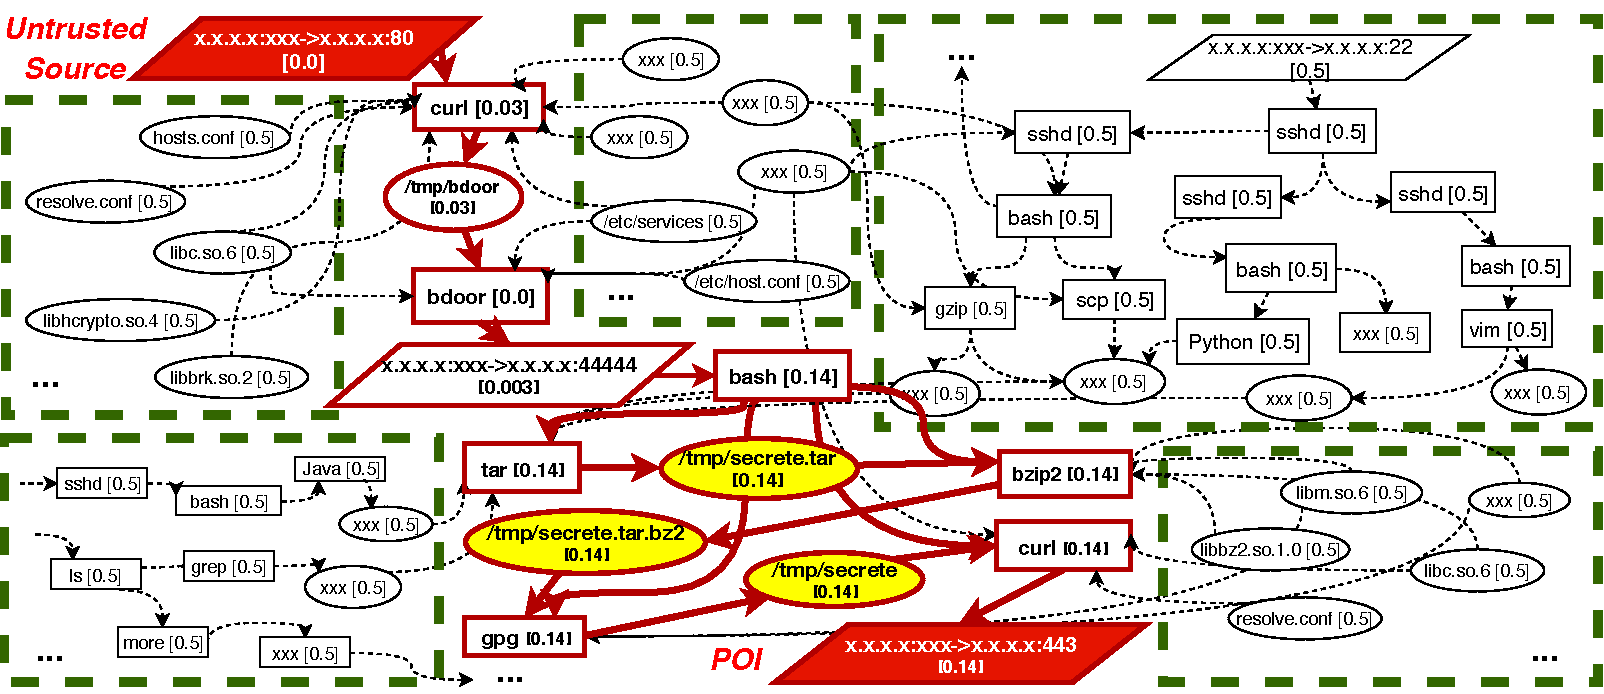
\includegraphics[width=\textwidth, keepaspectratio]{figs/overview.pdf}
    \caption{Partial dependency graph of an attack that downloads a malicious file and hides the file by renaming it (rectangles for processes, ovals for files, parallelograms for network connections).
    The complete dependency graph constructed from the POI event (renaming to \incode{user/file.txt}) via backward causality analysis contains $194,208$ nodes and $3,273,769$ edges.
    %
    The critical component identified by \tool is colored in dark black, which contains $10$ nodes (including $2$ attack entries) and $12$ edges (these edges are all critical edges).
    As can be seen, \tool significantly reduces the size of the dependency graph while preserving the critical attack information.
    }

   % \vspace{2mm}
    \label{fig:motivate}
\end{figure*}


\section{Background and Motivation}

\subsection{System Monitoring}
\label{subsec:system-monitoring}

System monitoring collects auditing events about system calls that are crucial in security analysis, describing the interactions among system entities.
As shown in previous studies~\cite{backtracking,backtracking2,taser,wormlog,gao2018saql,gao2018aiql,mcitracking,logtracking,liu2018priotracker,hassan2019nodoze}, on mainstream operating systems (Windows, Linux, and Mac OS), system entities in most cases are files, processes, and network connections,
and the collected system calls are mapped to three major types of system events:
(1) file access, 
(2) processes creation and destruction, and 
(3) network access. 
Following the established trend, in this work, we consider \emph{system entities} as \emph{files}, \emph{processes}, and \emph{network connections}. 
We consider a \emph{system event} as the interaction between two system entities represented as \emph{$\langle$subject, operation, object$\rangle$}. Subjects are processes originating from software applications (\eg Chrome), and objects can be files, processes, and network connections. 
We categorize system events into three types according to the types of their object entities, namely \emph{file events}, \emph{process events}, and \emph{network events}.
Both entities and events have critical security-related
attributes (\cref{tab:entity-attributes,tab:event-attributes}).
Representative attributes of entities include file name, process executable name, IP, and port.
%unique identifiers to distinguish entities (\eg file path, process name and PID, IP and port).
Representative attributes of events include event origins (\eg start time/end time) and operations (\eg file read/write).
%, and other security-related properties (\eg failure code). 
%(\eg system call return code).

%%%%%%%%%%%%%%%%%%%%%%%%%%
\subsection{Causality Analysis}
\label{subsec:causality-analysis}

Causality analysis~\cite{backtracking,backtracking2,taser,intrusionrecovery,liu2018priotracker,mcitracking,hassan2019nodoze,ma2016protracer} analyzes the auditing events to infer their dependencies 
%among system entities 
and present the dependencies as a directed graph.
%
In the dependency graph $G(E,V)$, a node $v \in V$ represents a process, a file, or a network connection.
An edge $e(u, v) \in E$ indicates a system auditing event that involves two entities $u$ and $v$ (\eg process creation, file read or write, and network access), and its direction (from the source node $u$ to the sink node $v$) indicates the direction of data flow.
Each edge is associated with a time window, $tw(e)$.
We use $ts(e)$ and $te(e)$ to represent the start time and the end time of $e$.
Formally, in the dependency graph, for two events $e_1(u_1, v_1) $ and $e_2(u_2, v_2)$, there exists causal dependency between $e_1$ and $e_2$ if $v_1 = u_2$ and $ts(e_1) < te(e_2)$.

Causality analysis enables two important security applications:
(1) \emph{backward causality analysis} that identifies entry points of attacks, and (2) \emph{forward causality analysis} that investigates ramifications of attacks.
Given a POI event $e_s(u,v)$, a backward causality analysis traces back from the source node $u$ to find all events that have causal dependencies on $u$,
and a forward causality analysis traces forward from the sink node $v$ to find all events on which $v$ has causal dependencies.


\begin{table}[t]
	\centering
	\caption{Representative attributes of system entities}
	\label{tab:entity-attributes}
	\resizebox{0.44\textwidth}{!}{%
		\begin{tabular}{l|l|l}
			\hline
			\textbf{Entity}             & \textbf{Attributes}    & \textbf{Shape in Graph} \\ \hline
			File               & Name, Path          & Ellipse        \\
			Process            & PID, Name, User, Cmd  & Square         \\
			Network Connection & IP, Port, Protocol   & Parallelogram  \\ \hline
		\end{tabular}%
	}
\end{table}


% \eat{
% \begin{table}[!t]
% 	\centering
% 	\caption{Representative attributes of system entities}\label{tab:entity-attributes}
% 	\begin{adjustbox}{0.45\textwidth}
% 		\begin{tabular}{|l|l|}
% 			\hline
% 			\textbf{Entity}		&\textbf{Attributes}\\\hline
% 			File				&Path\\\hline
% 			Process			&PID, Name, User, Cmd\\\hline
% 			Network Connection	& IP, Port, Protocol \\\hline
% 		\end{tabular}
% 	\end{adjustbox}
% 	%	\vspace*{-2ex}

% 	\vspace*{1ex}
% \end{table}
% }
\begin{table}[!t]
	\centering
	\caption{Representative attributes of system events}
	\label{tab:event-attributes}
	\begin{adjustbox}{width=0.44\textwidth}
		\begin{tabular}{l|l}
			\hline
			\textbf{Operation}		& Read/Write, Execute, Start/End\\\hline
			\textbf{Time}		& Start Time/End Time, Duration\\\hline
			\textbf{Misc.}		& Subject ID, Object ID, Data Amount, Failure Code\\\hline
		\end{tabular}
	\end{adjustbox}
	%	\vspace*{-2ex}

	%	\vspace*{1ex}
\end{table}


\eat{
\begin{table}[!t]
	\centering
	\caption{Representative attributes of system events}\label{tab1:event-attributes}
	\begin{adjustbox}{width=0.48\textwidth}
		\begin{tabular}{|l|l|}
			\hline
			Operation		& Read/Write, Execute, Start/End, Rename/Delete.\\\hline
			Time/Sequence		& Start Time/End Time, Event Sequence\\\hline
			Misc.		& Subject ID, Object ID, Failure Code\\\hline
		\end{tabular}
	\end{adjustbox}
	%	\vspace*{-2ex}

		\vspace*{1ex}
\end{table}
}



%%%%%%%%%%%%%%%%%%%%%%%%
\subsection{Motivating Example}
\label{subsec:motivating-example}

\cref{fig:motivate} shows a partial dependency graph of a 
%real 
file hiding activity: 
a suspicious script \incode{mal.sh} is executed to download a malicious file \incode{mal} from a remote host \incode{192.1.1.254}. The file is then moved to \incode {user/mal} and renamed to \incode{user/file.txt}.
%
Given a POI event which renames the file to \incode{user/file.txt}, the dependency graph produced by backward causality analysis 
%from the POI event 
contains $194,208$ nodes and $3,273,769$ edges.
%(the original dependency graph constructed from system audit logs contains $784$ nodes and $6,911$ edges).
The critical edges and attack entries (\incode{192.1.1.254}, \incode{mal.sh}) that represent the attack sequence are colored in dark black.
%
The goal of attack investigation is to inspect the dependency graph to
reveal critical edges and attack entries of the attack.
%obtain the context information (attack entries and critical edges) of the attack.
%the root cause node of the POI, reveal the attack edges, and reconstruct the attack sequence from the massive number of irrelevant nodes and edges.


\myparatight{Challenges}
As observed in \cref{fig:motivate}, attack investigation is a process of \emph{finding a needle in a haystack}: 
a limited number of critical edges (\ie $12$) are buried in an overwhelmingly large number ($\sim 3$ million) of non-critical edges (\ie less-important dependencies),
and same for attack entries (\ie $2$ out of $\sim 35K$ irrelevant entry nodes).
%and normal program execution like Java and Python), 
%and same for the root cause node (\ie $1$) is buried in many other entry nodes (\ie $80$;
%\eg ssh logging in).
%\eg network connections for browser updating and ssh logging in). 
% Existing approaches~\cite{backtracking,backtracking2,taser,intrusionrecovery,liu2018priotracker} require intensive efforts of manually inspecting these edges and nodes for revealing critical edges, identifying root cause nodes, and reconstructing the attack sequence.
% As such, how to automate this process for effectively finding a needle in a haystack becomes a key challenge.
When existing techniques, such as PrioTracker~\cite{liu2018priotracker} and NoDoze~\cite{hassan2019nodoze}, are applied to identify these critical edges, they achieve poor performance.
PrioTracker relies on the fanout value of a node to prioritize the edges.
As the process \incode{bash} has a high fanout value and the critical edges are connected with it, PrioTracker needs a higher threshold to keep the critical edges, and thus producing a dependency graph with $114,614$ edges.
NoDoze relies on an execution profile to filter irrelevant events.
However, due to the complex nature of computer systems, it is almost impossible to obtain an execution profile that covers most common system behaviors.
Specifically, there are many edges introduced by the irrelevant process \incode{grep}, which is not frequently observed when the execution profile is trained.
Such rare benign events cause NoDoze to produce a dependency graph with $37,251$ edges.


\myparatight{Using \tool to Identify Critical Component}
% To remove less-important dependencies introduced by irrelevant system activities, \tool identifies the critical component, a subgraph that consists of mainly 
% %relevant dependencies,
% critical edges and attack entries,
% by (1) computing dependency weights for edges and computing dependency impacts for entry nodes, (2) ranking entry nodes based on their dependency impacts, and (3) performing forward causality analysis from the top-ranked entry nodes to filter out irrelevant parts of the graph.
\tool first divides the entry nodes into $3$ categories (\ie network connections, files, and processes), and ranks the entry nodes in each category.
Here, \tool ranks the IP \incode{192.1.1.254} for \incode{mal} downloading as top $1$, the malicious script \incode{mal.sh} and the executable \incode{/bin/mv}
%for the process \incode{mv}
as top $1$ and top $2$.
By performing forward causality analysis from top-ranked entry nodes and taking the overlap, \tool filters out most less-important dependencies ($\sim 3$ million) and identifies the critical component (colored in dark black; $10$ nodes, $12$ edges) that preserves all critical edges and attack entries.
\textit{Note that PrioTracker's graph is $\sim141\times$ bigger than \tool's graph, and NoDoze's graph is $\sim46\times$ bigger than the \tool's graph}.



\begin{figure*}[!ht]
    \centering
    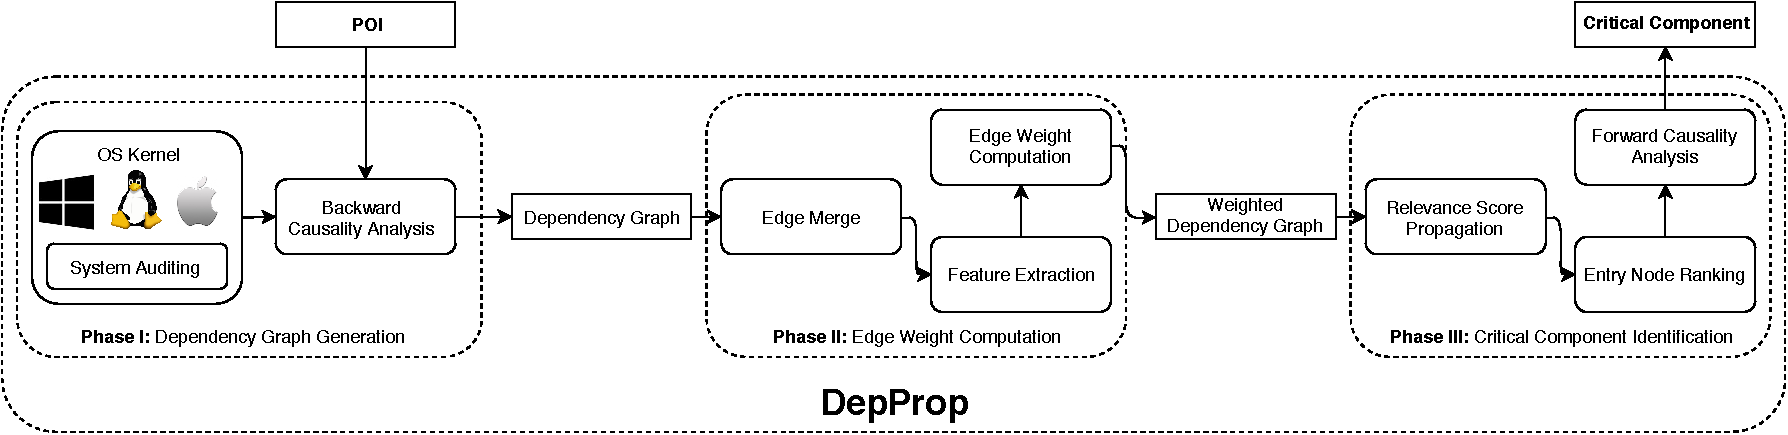
\includegraphics[width=0.95\textwidth,clip]{figs/architecture.pdf}
  %  \vspace{3mm}
    \caption{The architecture of \tool}
  %  \vspace{2mm}
    \label{fig:overview}
%    \vspace*{-1ex}
\end{figure*}


\section{Overview and Threat Model}
\label{sec:overview}

% https://drive.google.com/file/d/1HKHxWAoQWrw-ZGfvF3AJuEUhGcIF-BCy/view?usp=sharing
\cref{fig:overview} illustrates the architecture of \tool. 
\tool consists of three phases: (1) dependency graph generation, (2) graph preprocessing \& discriminative weight computation, and (3) attack investigation.
In Phase I, 
\tool leverages mature system auditing tools (\eg auditd~\cite{auditd}, ETW~\cite{etw}, DTrace~\cite{dtrace}, and Sysdig~\cite{sysdig}) to collect system-level audit logs about system calls.
Given a POI event, \tool parses the collected logs and performs causality analysis~\cite{backtracking,backtracking2} to generate the dependency graph for the event (\cref{subsec:graph-generation}).
%
In Phase II, \tool preprocesses the graph by merging the same type of edges between two nodes that occur within a time window threshold to reduce the graph size and splitting the nodes to remove parallel edges. 
This process transforms the large dependency graph into a simple directed graph (\cref{subsec:graph-preprocessing}), which is easier for weight computation and reputation propagation.
To compute discriminative weights for edges so that critical edges can be easily revealed from non-critical edges,
%To produce a weighted dependency graph such that critical edges
%(\ie edges that reveal the attack provenance) 
%can be easily revealed from non-critical edges using their edge weights, 
for each edge, \tool extracts three novel features that model the 
%importance of the event edge with respect to the POI event
%correlation between the event edge and the POI event 
impact of the event edge on the POI event
from three aspects: time aspect, data amount aspect, and structure aspect (\cref{subsec:feature-extraction}). 
\tool then employs a novel 
\emph{discriminative feature projection scheme}
%\emph{local feature projection mechanism}
to combine the three features into a single discriminative weight (\cref{subsec:weight-computation}).
%
%
In Phase III, \tool propagates reputation from entry nodes to the POI along the weighted edges to infer the POI reputation.
The 
%inferred 
POI reputation will be used to identify the root cause nodes and determine the POI trustworthiness/suspiciousness. 
Furthermore, \tool provides a suggested range of threshold values based on the edge weights, which will be used to reconstruct the attack sequence.





\myparatight{Threat Model}
Our threat model follows the threat model of previous work on system monitoring~\cite{backtracking,backtracking2,loggc,trustkernel,gao2018aiql,gao2018saql,liu2018priotracker,hassan2019nodoze}. 
We assume that the system monitoring data collected from kernel space~\cite{auditd,etw,dtrace,sysdig} is not tampered, and that the kernel is trusted.
Any kernel-level attack that deliberately compromises security auditing systems is beyond the scope of this work.



\eat{
The attacker executes APT attacks involving multiple steps such as target discovery and data exfiltration. We assume an outside attacker that attacks the system remotely (from outside of the system). Thus, the attacker either utilizes the vulnerabilities in the system or convinces the user to download a file. The main goal of the attacker is to inject her malicious files into the victim’s system without being detected. In this work, we assume the attacker does not know how the proposed reputation system operates, and hence we do not consider the potential attacks against the reputation system. 

% We do consider that insiders or external attackers have full knowledge of the deployed \tool queries and the anomaly models. 
}

\section{Design of \tool}
\label{sec:approach}

% In this section, we present \tool in detail.

In this section, we present the design details of each phase shown in \cref{fig:architecture}.
Specifically, \cref{subsec:phase1} describes how \tool collects system audit logs and generates a dependency graph,
\cref{subsec:phase2} describes how \tool computes the weight for each edge in the dependency graph to generate a weighted dependency graph,
and \cref{subsec:phase3} describes how \tool identifies critical components based on the weighted dependency graph.




\subsection{Dependency Graph Generation}
\label{subsec:phase1}


In Phase I, \tool leverages system monitoring to collect auditing logs of system activities and applies causality analysis on the collected logs to generate a dependency graph based on the given POI events.



\subsubsection{System Auditing}
\label{subsubsec:system-auditing}

\tool leverages mature system auditing frameworks~\cite{auditd,etw,dtrace,sysdig} to collect system audit logs about system calls from the kernel. 
\tool then parses the collected logs to build a \emph{global} system dependency graph, where nodes represent system entities and edges represent system (call) events. 
In particular, \tool focuses on three types of system entities/events: 
(i) file access, 
(ii) process creation and destruction, and
(iii) network access.
%
\cref{tab:events} shows the representative system calls (in Linux) processed by \tool.
Failed system calls are filtered out by \tool, as processing them will cause false dependencies among events.
\cref{tab:entity-attributes,tab:event-attributes} show the representative attributes of entities and events extracted by \tool.
%
Following the existing work~\cite{liu2018priotracker,gao2018aiql,gao2018saql}, to uniquely identify entities,
for a process entity, we use the process name and PID as its unique identifier.
For a file entity, we use the absolute path as its unique identifier. 
For a network 
%socket 
connection entity, we use 5-tuple (\emph{$\langle$srcip, srcport, dstip, dstport, protocol$\rangle$)} as a network 
connection's unique identifier. 
% as processes usually communicate with some servers using different network connections but with the same IPs and ports, treating these connections differently greatly increases the amount of data we trace and such granularity is not required in most of the cases~\cite{liu2018priotracker,gao2018aiql,gao2018saql}. Thus, 
Failing to distinguish different entities causes problems in relating events to entities and tracking the dependencies among events.




\subsubsection{Backward Causality Analysis}
\label{subsubsec:backward-causality}

Given a POI event, \tool performs backward causality analysis (\cref{subsec:causality-analysis}) to generate a \emph{local} backward dependency graph $G_d$ for the POI event.
%
Briefly speaking, backward causality analysis adds the POI event to a queue, and repeats the process of finding eligible incoming edges of the edges/events (\ie incoming edges of the source nodes of edges) in the queue until the queue is empty. 
The output of Phase I is a backward dependency graph that only contains system events (and associated entities) and that are causally dependent on the POI event.






%%%%%%%%%%%%%%%%%%%%%%%%%%%%%%%%%%%%%%%%%%%%

\subsection{Dependency Weight Computation}
\label{subsec:phase2}

In Phase II, \tool first merges parallel edges between two nodes in the dependency graphs, and compute the weights of the edges using three types of features, including timing, data flow amount, and node degree.
Based on these features, \tool clusters edges into two groups and leverages LDA to compute a weight score such that the weight differences of the edges in these two groups are maximized.
The final step of the weight computation is to normalize the weights of all outgoing edges for each node. 
This step mitigates the weight degradation for the edges that are far from the POI events. 



\subsubsection{Edge Merge}
\label{subsubsec:edge-merge}

The dependency graph produced by causality analysis often has many parallel edges between two nodes~\cite{reduction}.
The reason is that OS typically finishes a read/write task (\eg file read/write) by distributing the data proportionally to multiple system calls.
% and each system call processes only a portion of data.
% Although these edges preserves causal dependency~\cite{backtracking,reduction},
% they create complication in propagating reputations: 
% the reputation of the same node will be propagated multiple times.
% that proposed Causality Preserved Reduction (CPR)
Inspired by the recent work for dependency graph reduction~\cite{reduction}, \tool merges the edges between two nodes if the time differences of these edges are smaller than a given threshold. 
% As shown in~\cite{reduction}, CPR does not work well for processes that have many interleaved read and write system calls, which introduces excessive causality.
% As such, \tool adopts a more aggressive approach: for edges with the same direction (\ie representing read or write) between two nodes, 
%(\eg file reads from \incode{read} or network reads from \incode{recvfrom}), 
% \tool will merge them into one edge if the time differences of these edges are smaller than a given threshold. 
We tried different values for the merge threshold and selected 10s, as it gives reasonable results in merging system calls for file manipulations, file transfers, and network communications, which is consistent with~\cite{reduction}.
% Since such merge is performed after the dependency graph generation, all the dependencies among the merged edges are still preserved.
% with the time windows of certain edges merged.
%We tried different values, and 10s gives reasonable results in merging system calls for file content manipulation, which is consistent with [56]
%Empirically, we set the threshold as 10 seconds, which is large enough for most processes to finish file transfers and network communications in modern computers. 



\eat{
\myparatight{Node Split}
After the edge merge, the dependency graph may still have parallel edges (\ie edges indicating read or write from different system calls).
For example, a process may receive data from a network socket via both \incode{read} and \incode{recvfrom}.
% Although we merge edges within 10 seconds, it is possible that there are still parallel edges because of some long-running file transfers.
These parallel edges create complications for weight computation: for a node, some of its incoming edges' time windows may violate the causal dependencies on the outgoing edges.

To address the problem, 
\tool first enumerates all node pairs that have parallel edges.
For a node pair $(u,v)$ with parallel edges from $u$ to $v$,
\tool splits $u$ into multiple copies and assigns each copy to one parallel edge, so that each copy only has one outgoing edge to $v$. The copies of $u$ also inherit all $u$'s incoming edges that have causal dependencies on $u$'s outgoing edges.
The output is a simple directed dependency graph without parallel edges.
}




%%%%%%%%%%%%%%%%%%%%%%%%%%%%%%%%%%%%%%%%%%%%

\subsubsection{Feature Extraction}
\label{subsubsec:feature-extraction}
For each edge, \tool extracts three features to compute a dependency weight,  
enabling \tool to address scenarios where a single feature (\eg data flows) cannot be used to distinguish critical edges.
% models the correlation between the edge and the POI event.


%  Thus, DepImpact synergistically combines 3 features, and our normalization ensures that each edge is assigned a local weight w.r.t the outgoing edges that have the same source node, 

%The dependency weights are essential to revealing critical edges:
% An edge with a higher dependency weight implies more relevance to the POI event, and is more likely to be a critical edge.
%

\myparatight{Data Flow Relevance $f_{S(e)}$}
Intuitively, edges that have similar data flow amount as the data size of the entities in the POI event are more likely to be relevant.
As such, we design feature $f_{D(e)}$ to model the data flow relevance of an edge $e(u, v)$ to the POI event:

\begin{equation}
\label{eq:data-feature}
    f_{S(e)} = 1/(\mid s_{e} - s_{e_s}\mid + \alpha)
\end{equation}
where $s_{e}$ and $s_{e_s}$ represent the data 
%size 
flow amount associated with the edge $e$ and the POI event $e_s$.
The smaller the difference $\mid s_{e} - s_{e_s}\mid$, the higher the data flow relevance $f_{S(e)}$.
%
Note that we use a small positive number $\alpha$ (we set $\alpha = 1\mathrm{e}{-4}$) to handle the special case when $e$ is the POI event: POI event has the highest feature value $f_{S(e_s)} = 1/\alpha$.
%In our design, we set $\alpha = 1\mathrm{e}{-4}$.


\myparatight{Temporal Relevance $ f_{T(e)}$}
Intuitively, edges that occurred at relatively the same time are more likely to be relevant.
As such, we design feature $f_{T(e)}$ to model the temporal relevance of an edge $e(u,v)$ to the POI event:

\begin{equation}
\label{eq:time-feature}
    f_{T(e)} = \ln(1 + 1/\mid t_{e} - t_{e_s}\mid)
\end{equation}
where $t_{(e)}$ and $t_{e_s}$ represent the timestamp values (we use the event end time) of the edge $e$ and the POI event $e_s$. 
The smaller the difference $\mid t_{e} - t_{e_s}\mid$, the higher the temporal relevance $f_{T(e)}$.
%
To handle the special case when $e$ is the POI event (\ie $\mid t_{e} - t_{e_s}\mid = 0$), we use one tenth of the minimal time unit (nanosecond) in the audit logging framework (\ie $1\mathrm{e}{\mbox{-}10}$) to compute its feature value: $f_{T(e_s)} = ln(1 + 1\mathrm{e}{10})$. 
This ensures that the POI event has the highest feature value.


\myparatight{Concentration Ratio $f_{C(e)}$} 
In the backward causality analysis, if the number of source nodes that can be traced from a node $v$ is 1 (\ie only one incoming edge from $v$), we say that the dependency represented by this edge is highly concentrated for $v$.
Also, we would like to give higher weights to the node that can be reached from multiple paths in the backward direction.
Thus, we define the \emph{concentration ratio} for the edge $e(u, v)$ as:

\begin{equation}
    \label{eq:structure-feature}
    f_{C(e)} = OutDegree(v)/InDegree(v)
\end{equation}
    
Here, $InDegree(v)$ and $OutDegree(v)$ represent the in-degree and out-degree of the sink node $v$.

\eat{
One important category of non-critical edges that often appear in a causal graph are events that access system libraries~\cite{reduction,reduction2}. These edges are often associated with considerable data amount and occur at various timestamps, and hence using only $f_{S(e)}$  and $f_{T(e)}$ is less effective in revealing critical edges from them.
To address this challenge, we observe that most system library nodes are source nodes in the corresponding edges and do not have any incoming edges.
Another category of non-critical edges are events that involve long-running processes as source nodes, which often have few incoming edges but many outgoing edges.}


% discussion






%
%However, it is important to note that the proposed features are by no means absolute or comprehensive.
%The design of \tool allows the security analyst to adjust proposed features and incorporate new features according to specific forensic investigation needs.




%%%%%%%%%%%%%%%%%%%%%%%%%%%%%%%%%%%%%%%%%%%%
%%%%%%%%%%%%%%%%%%%%%%%%%%%%%%%%%%%%%%%%%%%%
%%%%%%%%%%%%%%%%%%%%%%%%%%%%%%%%%%%%%%%%%%%%

\subsubsection{Dependency Weight Computation}
\label{subsubsec:weight-computation}

% http://www.sci.utah.edu/~shireen/pdfs/tutorials/Elhabian_LDA09.pdf

To compute a dependency weight from the features, \tool leverages linear projection that is known for high interpretability and low computational cost~\cite{friedman2001elements}.
Instead of directly taking the average,
%(equivalent to projecting onto unit vector $[1\; 1\; \frac{1}{\sqrt{3}}]^T$), 
\tool employs a \emph{discriminative feature projection scheme} based on Linear Discriminant Analysis (LDA)~\cite{Mika99fisherdiscriminant} to compute a projection vector to maximize the differences between critical edges and non-critical edges, with critical edges assigned with higher weights.
% In this way, the projected weights of critical edges and non-critical edges are maximally separated, and critical edges 
% %generally 
% have higher weights than non-critical edges.
%
Next, we present the scheme in detail.



\myparatight{Step 1: Edge Clustering}
In the first step, \tool leverages clustering to separate edges into two groups: one is likely to contain critical edges, and the other for non-critical edges.
%
%Note that as shown in \pgao{\cref{x}}, due to imperfections of features, the clustering results may be noisy and hence cannot be straightforwardly used to identify critical component graph. 
%
Specifically, \tool first normalizes features to 0-1 range~\cite{friedman2001elements}, and then employs Multi-KMeans++ clustering algorithm~\cite{Arthur:2007:KAC:1283383.1283494}, which improves over standard KMeans algorithm on initial seeds selection and clustering robustness.
% KMeans clustering algorithm aims to partition the points into $k$ clusters such that each point belongs to the cluster with the nearest center.
% Based upon KMeans, KMeans++ improves the initial seeds selection to avoid poor clustering.
% Multi-KMeans++ is a meta algorithm that performs $n$ runs of KMeans++ and then chooses the best clustering that has the lowest distance variance over all clusters.
We choose $k=2$ since we want to cluster edges into two groups, as required by LDA.
We experimented a range of values for $n$ ($[5, 30]$) and chose $n=20$ as it delivers the best clustering results without much overhead.
While the clustering results can be used to directly distinguish critical and non-critical edges, such approach will suffer from the same problem as global weights~\cite{hassan2019nodoze}, which is shown to be ineffective in \cref{subsec:rq1}.

%based on our empirical analysis.




\myparatight{Step 2: Discriminative Feature Projection}
Given two groups of edges, \tool leverages Linear Discriminant Analysis (LDA)~\cite{Mika99fisherdiscriminant} to compute an optimal projection vector that maximizes the separation between group projections.
%
%Briefly speaking, LDA seeks to reduce the dimensionality of data while preserving as much of the group discriminatory information as possible.
LDA finds the optimal projection plane such that the projected points in the same group are close to each other, and the projected points in different groups are far from each other.
%
Formally, LDA finds the projection vector $\omega$ that maximizes the Fisher criterion, $J(\omega) = \frac{\omega^TS_b\omega}{\omega^TS_w\omega}$, where $S_b$ and $S_w$ are between-group scatter matrix and within-group scatter matrix, respectively. 
%
Solving the optimization problem yields:

\begin{equation}
    \label{eq:lda-solution}
    \omega^* = \argmax J(\omega) = S_w^{-1}(\mu_1-\mu_2)
\end{equation}

Denote the solution to \cref{eq:lda-solution} as $\omega^{*} = [\omega^{*}_{S}\; \omega^{*}_{T}\; \omega^{*}_{C}]^T$.
For an edge $e$, its unnormalized weight $W_{e_{UN}}$ is computed as:

\begin{equation}
    \label{eq:projection}
    W_{e_{UN}} = \omega^{*}_{S} f_{S(e)} + \omega^{*}_{T} f_{T(e)} + \omega^{*}_{C} f_{C(e)}
\end{equation}

One remaining issue is that \cref{eq:lda-solution} does not guarantee the direction of the projection vector, and it might be possible that 
%negative projected weights and 
critical edges have lower weights than non-critical edges.
To address the issue, we leverage the observation that, in most cases, the number of critical edges is significantly less than the number of non-critical edges (as can be seen from attack cases in~\cref{subsec:evalsetup}).
Specifically, we negate the direction of the projection vector if the average of the projected weights for a smaller edge group (likely to be the group of critical edges) is smaller.
%
As shown in \cref{subsec:rq3}, compared to the naive approach of taking the average of features (the average-projection approach), our feature projection scheme preserves as much of the group discriminatory information as possible and leads to better performance for entry node ranking.
%(\ie entry nodes that are more relevant to POI are ranked upfront)




\eat{
Formally speaking, for each node $v$, the feature vectors $\{x\}$ of its $N$ incoming edges are clustered into two groups, $g_1$ (containing $N_1$ edges) and $g_2$ (containing $N_2$ edges), with group mean vectors: $\mu_1 = \frac{1}{N_1}\sum_{x \in g_1} x$, $\mu_2 = \frac{1}{N_2}\sum_{x\in g_2} x$, $N_1 + N_2 = N$.
The between-group scatter matrix is defined as: $S_b = (\mu_1 - \mu_2)(\mu_1 - \mu_2)^T$.
The within-group scatter matrix is defined as: $S_w = \sum_{x\in g_i}(x-\mu_i)(x-\mu_i)^T$.
}

\eat{
Note that sometimes, the projected weights may contain non-positive values. To be amenable to the next step, in such condition, we shift all the projected weights to make them positive.
}


\eat{
The applicability of \cref{eq:lda-solution} requires that $S_w$ is nonsingular (\ie $S_w^{-1}$ exists).
However, this criterion may be violated quite often in our problem context, due to the large imbalance between the number of critical edges and the number of non-critical edges.
Furthermore, standard LDA only ensures that the projected values of different groups are maximally separated, rather than guaranteeing which group has higher projected values, while our goal is to make critical edges have higher weights than non-critical edges.

Recognizing such limitations, we \emph{extend the standard LDA} from the following two aspects.

\emph{(a) Handling singular $S_w$:}
When $S_w$ is singular, we select the projection vector
%(we normalize it first) 
from the following two candidates that results in a larger Fisher criterion numerator (\ie $\omega^TS_b\omega$):

\begin{itemize}[noitemsep, topsep=1pt, partopsep=1pt, listparindent=\parindent, leftmargin=*]

    \item $S_w^{+}(\mu_1-\mu_2)$, where $S_w^{+}$ is the Moore-Penrose~\cite{albert1972regression} inverse of $S_w$. 
    %When $S_w$ is non-singular, $S_w^{+} = S_w^{-1}$.
    
    \item $\mu_1-\mu_2$ (\ie the direction of group mean difference)
    %difference between group means)
\end{itemize}

\emph{(b) Correcting the projection vector direction:}
We correct the direction of the projection vector (\ie negate), if critical edges have lower projected values than non-critical edges.
Note that this problem is fundamentally challenging, since we do not have labels for critical edges and thus we do not know which group contains critical edges. 
We approach this problem using a set of heuristics:

\begin{enumerate}[label=\Roman*, noitemsep, topsep=1pt, partopsep=1pt, listparindent=\parindent, leftmargin=*]

\item If all three dimensions of the projection vector are non-positive, negate.
\item Else if all three dimensions of the projection vector are non-negative, do not negate.
\item Else, 
%If the projection vector has both negative dimensions and positive dimensions, 
if the group with a smaller size has a smaller projected mean, negate.
This is based on the insight that the number of critical edges is smaller than the number of non-critical edges in most cases.

\end{enumerate}
}




\myparatight{Step 3: Edge Weight Normalization}
For an edge $e(u, v)$, we normalize its projected weight by the sum of weights of all outgoing edges of the source node $u$:

\begin{equation}
    \label{eq:local-weight-normalization}
    W_e = W_{e_{UN}}/\sum_{e' \in outgoingEdge(u)} W_{e'_{UN}}
\end{equation}

The rationale behind is to ensure that for each node, the weights of all its outgoing edges are in the range $[0.0, 1.0]$ and the sum of the weights is equal to $1.0$.
%
Coupled with our score propagation scheme for dependency impact (\cref{subsec:phase3}), such way of normalization ensures that (1) the dependency impact of any node does not exceed the maximum dependency impact of its child nodes, and (2) the dependency impact of any node does not exceed the dependency impact of the nodes in the POI event (\ie $1.0$).
%, and guarantee the convergence of reputation propagation.
%
The output of Phase II is a weighted backward dependency graph for the POI event, in which the dependency weights encode the differences between critical edges and non-critical edges.



%%%%%%%%%%%%%%%%%%%%%%%%%%%%%%%%%%%%%%%%%%%%

\subsection{Phase III: Critical Component Identification}
\label{subsec:phase3}

\subsection{Phase III: Critical Component Identification}
\label{subsec:phase3}

\input{algs/relevance-propagation}


\subsubsection{Relevance Score Propagation}
\label{subsubsec:propagation}

Given a weighted dependency graph, \tool propagates the relevance score from POI to all other nodes along the weighted edges. 
Formally speaking, the relevance score of a node is a real number in $[0, 1]$ that models the relevance of the node to POI. 
For POI node, its relevance score is $1$.

%
For a node $u$, its relevance score is iteratively updated by the scores of its child nodes: 
%To prevent the fast degredation of scores, instead of a distribution fashion, \tool updates a node $u$'s relevance score using an inheritance fashion:

\begin{equation}
    \label{eq:reputation}
     R_{u} =\sum_{v \in childNodes(u)} R_{v}*W_{e(u,v)}
\end{equation}
where $W_{e(u,v)}$ represents the normalized weight of edge $e(u,v)$ as computed in \cref{eq:local-weight-normalization}.
Such update mechanism guarantees that the score of any node does not exceed the maximum score of its child nodes, and the score of any node does not exceed the score of POI node (\ie $1$).
Furthermore, compared to the distribution-based score propagation algorithms like PageRank~\cite{pagerank}, our scheme preserves the scores along long dependency paths and prevents them from fast degradation.



\cref{alg:relevance-propagation} illustrates our relevance score propagation algorithm. 
In each iteration, the algorithm updates the relevance score of each node by taking the weighted sum of the corresponding child nodes (Line 10), and computes the sum of score differences for all nodes (Line 11).
The propagation terminates when the aggregate difference between the current iteration and the previous iteration is smaller than a threshold, $\delta$ (Line 2), indicating that the scores of all nodes become stable.
Empirically, we set $\delta = 1e-13$.
Note that the reputation of POI node remains unchanged (Line 1, Line 6).



\eat{
A node $v$ in the dependency graph receives its reputation by inheriting the weighted reputation from all of its parent nodes (Lines 7-12).
Note that if we adopt a distribution fashion that ensures the sum of reputations for $v$'s children nodes to be equal to $v$'s reputation,
then the reputation will degrade rapidly in a few hops, which does not work well for dependency graphs that often have many paths with many hops.
}



\subsubsection{Entry Node Ranking}
\label{subsubsec:entry-ranking}
After the relevance score has been propagated backward from POI to entry nodes, the next step is to rank the entry nodes based on their scores.
Entry nodes, by definition, are the nodes on the dependency graph that do not have incoming edges, and hence they denote the end of relevance score propagation.
The intuition behind is that entry nodes with higher scores are more likely to be related to POI, and thus their descendant nodes and associated edges are more likely to be include in the critical component that we want to identify.
By selecting the top ranked candidates and performing forward causality analysis to identify descendants, we are able to significantly prune the dependency graph and only retain the relevant parts. 

In the current design of \tool, we have a special treatment of system library nodes. 
As has been shown in prior work~\cite{reduction2}, system library files are typically loaded by certain processes, and do not have incoming edges on the dependency graph.
As the number of system library nodes could be potentially large, naively treating them all as entry nodes could add significant difficulties to entry nodes ranking and candidates selection, impairing the final results.
%not robust.
As such, for system library nodes, we take the process nodes that load them as entry nodes instead.
%
Specifically, in the current design, we classify entry nodes into three categories: (1) file entry node: file nodes that do not have incoming edges except system libraries; (2) process entry node: process nodes whose parent nodes are all system libraries; (3) network entry node: network nodes that do not have incoming edges. 
We then select top-$k$ ranked candidates from each category.


%  file entry  就是指除了 library 之外的file, ip entry 就是所有的 ip, process entry 就是 它的父亲如果都是library 那这个process 就被当作 entry


\eat{
Entry nodes are the nodes without incoming edges in the dependency graph. 
They are usually trusted sources such as official updates like Microsoft updater or Chrome updater (assigned high reputations), system libraries like libc (assigned neutral reputations), or suspicious sources like USB sticks or malicious websites (assigned with low reputations). For each trusted source, its initial reputation is set to $1.0$; for each suspicious source, its initial reputation is set to $0.0$. 
Additionally, since the system libraries will be used by both legitimate users and attackers, we cannot easily infer a node's nature from its correlations with the system libraries. Thus, the initial reputations of system libraries are set to $0.5$. 
However, \tool also allows security analysts to manually set the reputation for libraries.
}




\subsubsection{Forward Causality Analysis}
\label{subsubsec:forward-causality}
From the selected top ranked entry node candidates, \tool performs forward causality analysis until reaching POI. 
The process is similar to the backward causality analysis as illustrated in \cref{subsubsec:backward-causality}. 
%
As a final step, \tool identifies the overlap of the backward dependency graph and the forward dependency graph as the critical component for output.
Compared to the original large backward dependency graph, the critical component contains the parts of dependencies that are actually relevant to POI and its size is significantly reduced.
Furthermore, the critical component illustrates how the important information flows from entry node candidates to POI, which facilitates further forensic investigation.


\subsubsection{Relevance Score Propagation}
\label{subsubsec:propagation}

Given a weighted dependency graph, \tool propagates the relevance score from POI to all other nodes along the weighted edges. 
Formally speaking, the relevance score of a node is a real number in $[0, 1]$ that models the relevance of the node to POI. 
For POI node, its relevance score is $1$.

%
For a node $u$, its relevance score is iteratively updated by the scores of its child nodes: 
%To prevent the fast degredation of scores, instead of a distribution fashion, \tool updates a node $u$'s relevance score using an inheritance fashion:

\begin{equation}
    \label{eq:reputation}
     R_{u} =\sum_{v \in childNodes(u)} R_{v}*W_{e(u,v)}
\end{equation}
where $W_{e(u,v)}$ represents the normalized weight of edge $e(u,v)$ as computed in \cref{eq:local-weight-normalization}.
Such update mechanism guarantees that the score of any node does not exceed the maximum score of its child nodes, and the score of any node does not exceed the score of POI node (\ie $1$).
Furthermore, compared to the distribution-based score propagation algorithms like PageRank~\cite{pagerank}, our scheme preserves the scores along long dependency paths and prevents them from fast degradation.



\cref{alg:relevance-propagation} illustrates our relevance score propagation algorithm. 
In each iteration, the algorithm updates the relevance score of each node by taking the weighted sum of the corresponding child nodes (Line 10), and computes the sum of score differences for all nodes (Line 11).
The propagation terminates when the aggregate difference between the current iteration and the previous iteration is smaller than a threshold, $\delta$ (Line 2), indicating that the scores of all nodes become stable.
Empirically, we set $\delta = 1e-13$.
Note that the reputation of POI node remains unchanged (Line 1, Line 6).



\eat{
A node $v$ in the dependency graph receives its reputation by inheriting the weighted reputation from all of its parent nodes (Lines 7-12).
Note that if we adopt a distribution fashion that ensures the sum of reputations for $v$'s children nodes to be equal to $v$'s reputation,
then the reputation will degrade rapidly in a few hops, which does not work well for dependency graphs that often have many paths with many hops.
}



\subsubsection{Entry Node Ranking}
\label{subsubsec:entry-ranking}
After the relevance score has been propagated backward from POI to entry nodes, the next step is to rank the entry nodes based on their scores.
Entry nodes, by definition, are the nodes on the dependency graph that do not have incoming edges, and hence they denote the end of relevance score propagation.
The intuition behind is that entry nodes with higher scores are more likely to be related to POI, and thus their descendant nodes and associated edges are more likely to be include in the critical component that we want to identify.
By selecting the top ranked candidates and performing forward causality analysis to identify descendants, we are able to significantly prune the dependency graph and only retain the relevant parts. 

In the current design of \tool, we have a special treatment of system library nodes. 
As has been shown in prior work~\cite{reduction2}, system library files are typically loaded by certain processes, and do not have incoming edges on the dependency graph.
As the number of system library nodes could be potentially large, naively treating them all as entry nodes could add significant difficulties to entry nodes ranking and candidates selection, impairing the final results.
%not robust.
As such, for system library nodes, we take the process nodes that load them as entry nodes instead.
%
Specifically, in the current design, we classify entry nodes into three categories: (1) file entry node: file nodes that do not have incoming edges except system libraries; (2) process entry node: process nodes whose parent nodes are all system libraries; (3) network entry node: network nodes that do not have incoming edges. 
We then select top-$k$ ranked candidates from each category.


%  file entry  就是指除了 library 之外的file, ip entry 就是所有的 ip, process entry 就是 它的父亲如果都是library 那这个process 就被当作 entry


\eat{
Entry nodes are the nodes without incoming edges in the dependency graph. 
They are usually trusted sources such as official updates like Microsoft updater or Chrome updater (assigned high reputations), system libraries like libc (assigned neutral reputations), or suspicious sources like USB sticks or malicious websites (assigned with low reputations). For each trusted source, its initial reputation is set to $1.0$; for each suspicious source, its initial reputation is set to $0.0$. 
Additionally, since the system libraries will be used by both legitimate users and attackers, we cannot easily infer a node's nature from its correlations with the system libraries. Thus, the initial reputations of system libraries are set to $0.5$. 
However, \tool also allows security analysts to manually set the reputation for libraries.
}




\subsubsection{Forward Causality Analysis}
\label{subsubsec:forward-causality}
From the selected top ranked entry node candidates, \tool performs forward causality analysis until reaching POI. 
The process is similar to the backward causality analysis as illustrated in \cref{subsubsec:backward-causality}. 
%
As a final step, \tool identifies the overlap of the backward dependency graph and the forward dependency graph as the critical component for output.
Compared to the original large backward dependency graph, the critical component contains the parts of dependencies that are actually relevant to POI and its size is significantly reduced.
Furthermore, the critical component illustrates how the important information flows from entry node candidates to POI, which facilitates further forensic investigation.

\section{Evaluation}


We built \tool ($\sim$20K lines of code) upon Sysdig~\cite{sysdig}, and deployed our tool on 2 hosts to collect system auditing events and perform attack investigation. 
The deployed hosts have 12 active users with hundreds of processes, and are used for various types of daily tasks such as file manipulation, text editing, and software development, which are representative of real-world usage. 
During evaluation, the deployed hosts continue to resume their routine tasks to emulate the real-world deployment where irrelevant system activities and attack activities co-exist.
The routine tasks on these machines ensure that enough noise of irrelevant system activities is collected.
We performed a series of attacks based on known exploits~\cite{exploitdb,liu2018priotracker,kwon2018mci,reduction} in the deployed environment, and applied \tool to 
investigate these attacks, demonstrating the effectiveness of \tool.
In total, our evaluations used real system audit logs that contain \emph{100 million} events. 
%we collected \emph{100 million} real system auditing events for evaluation.
%Each attack is done with the time gap being at least 1 hour.

%Specifically, we 
We aim to answer the following research questions:

%\begin{itemize}[noitemsep, topsep=1pt, partopsep=1pt, listparindent=\parindent, leftmargin=*]
\begin{itemize}
\item \textbf{RQ1}: How effective is \tool in revealing attack sequences in comparison with other state-of-art techniques? 
\item \textbf{RQ2}: How do the top-ranked entry nodes affect \tool in revealing attack sequences?
\item \textbf{RQ3}: How effective is \tool in revealing attack entries?
\item \textbf{RQ4}: How efficient is \tool in investigating an attack?
\end{itemize}

% RQ1 aims to measure the effectiveness of using only weights for graph reduction.
% Its results will provide motivation for the design of \tool.
%  Its result evaluate the effectiveness of \tool for dependency graph reduction, which plays an essential role in addressing the challenges mentioned in \cref{sec:intro}.
RQ1 aims to evaluate the overall effectiveness of \tool in dependency graph reduction, and compare \tool with other state-of-the-art causality analysis techniques.
RQ2 aims to evaluate how the top-ranked entry nodes affect the effectiveness of \tool.
RQ3 aims to evaluate whether \tool consistently ranks the attack entries 
%as top-ranked nodes
upfront, and compare \tool with other baseline approaches.
RQ4 aims to measure the execution times of \tool and its variation, and compare \tool with other state-of-the-art causality analysis techniques.

\begin{table*}[!htb]
\centering
\caption{Statistics of dependency graphs generated for the 10 attacks}
\label{tab:stasticalSummary}
\resizebox{0.98\textwidth}{!}{
\begin{tabular}{crrrrrrr}
\hline
\textbf{Attack}      & \multicolumn{1}{c}{\textbf{Causality Analysis \# V}} & \multicolumn{1}{c}{\textbf{Causality Analysis \# E}} & \multicolumn{1}{c}{\textbf{Edge Merge \# V}} & \multicolumn{1}{c}{\textbf{Edge Merge \# E}} & \multicolumn{1}{c}{\textbf{Entry Nodes}} & \multicolumn{1}{c}{\textbf{Critical Edge}} & \multicolumn{1}{c}{\textbf{Attack Entries}} \\ \hline
Wget Executable      & 126                                                  & 673                                                  & 126                                          & 363                                          & 46                                        & 8                                          & 2                                             \\ 
Illegal Storage      & 8450                                                 & 93085                                                & 8450                                         & 62073                                        & 960                                       & 6                                          & 2                                             \\ 
Illegal Storage 2    & 42450                                                & 658913                                               & 42450                                        & 378326                                       & 3499                                      & 4                                          & 2                                             \\ 
Hide File            & 194208                                               & 6464098                                              & 194208                                       & 3273769                                      & 35203                                     & 12                                         & 2                                             \\ 
Steal Information    & 195636                                               & 6493626                                              & 195636                                       & 3291208                                      & 35213                                     & 4                                          & 2                                             \\ 
Backdoor Download    & 7510                                                 & 69479                                                & 7510                                         & 60390                                        & 157                                       & 8                                          & 2                                             \\ 
Annoying Server User & 114                                                  & 585                                                  & 114                                          & 318                                          & 34                                        & 8                                          & 2                                             \\ 
Shellshock           & 81                                                   & 10289                                                & 81                                           & 229                                          & 46                                        & 13                                         & 2                                             \\ 
Dataleak             & 174                                                  & 734                                                  & 174                                          & 459                                          & 95                                        & 11                                         & 1                                             \\ 
VPN Filter           & 549                                                  & 2986                                                 & 549                                          & 661                                          & 500                                       & 5                                          & 3                                             \\ 
\textbf{AVG}         & 44929.8                                              & 1379446.8                                            & 44929.8                                      & 706779.6                                     & 7575.3                                    & 7.9                                        & 2                                             \\ \hline
\end{tabular}
}
\end{table*}

\subsection{Evaluation Setup}
\label{subsec:evalsetup}
To evaluate \tool, we performed 10 attacks in the deployed environment: 7 attacks based on commonly used exploits and 3 multi-step intrusive attacks based on the Cyber Kill Chain framework~\cite{cyberkillchain} and CVE~\cite{cve}.
We then collected system auditing events for the attacks and applied \tool to analyze the events. 
\tool is executed on a server with an Intel(R) Xeon(R) CPU E5-2637 v4 (3.50GHz), 256GB RAM running 64bit Ubuntu 18.04.1.
Next, we describe the attacks in detail.



\subsubsection{Attacks Based on Commonly Used Exploits}
\label{subsub:benign-cases}
These 7 attacks are used as test cases in prior work~\cite{exploitdb,liu2018priotracker,kwon2018mci,reduction},
which consist of the following scenarios: 
%\begin{itemize}[noitemsep, topsep=1pt, partopsep=1pt, listparindent=\parindent, leftmargin=*]
\begin{itemize}
    \item \textit{Wget Executable}: A vulnerable server allows the attacker to download executable files using wget. The attacker downloads python scripts and executes the scripts.
    \item \textit{Illegal Storage}: A server administrator uses wget to download suspicious files to a user's home directory.
    \item \textit{Illegal Storage 2}: A server administrator uses curl to download suspicious files to a user's home directory.
    \item \textit{Hide File}: The goal of the attacker is to hide malicious file among the user's normal files. The attacker downloads the malicious script and hides it by changing its file name and location.
    \item \textit{Steal Information}: The attacker steals the user's sensitive information and writes the information to a hidden file.
    \item \textit{Backdoor Download}: A malicious insider uses the ping command to connect to the malicious server, and then downloads the backdoor script from the server and hides the script by renaming it.
    \item \textit{Annoying Server User}: 
    %A vulnerable server is used by multiple users. 
    The annoying user logs into other user's home directories on a vulnerable server and writes some garbage data to other user's files. 
\end{itemize}


\subsubsection{APT Attacks}
\label{subsubsec:attack-cases}

We performed five APT attacks that capture the important traits of APT attacks depicted from the Cyber Kill Chain framework~\cite{cyberkillchain}. 
Note that an APT attack consists of a series of steps, and some steps may not be captured by system monitoring (\eg user inputs and inter-process communications).
Such limitations can be addressed by employing more powerful auditing tools, but it is out of the scope of this paper.
Thus, we identified 10 key steps that are related to POI entities for our evaluations in the five APT attacks.


\myparatight{APT Attack 1: Zero-Day Penetration to Target Host}
The scenario emulates the attacker's behavior who penetrates the victim's host
leveraging previously unknown Zero-day attack. Zero-day vulnerabilities are
attack vectors that previously unknown to the community, therefore allow the
attacker to put their first step into their targets. In our case, we assume that
the {\tt bash} binary in victim's host is outdated and vulnerable to shellshock~\cite{shellshock}. The victim computer hosts web service that has
CGI written as BASH script. The attacker can run an arbitrary command when she
passes the specially crafted attack string as one of environment variable. Leveraging the vulnerability, the attacker runs a series of remote commands to
plant and run initial attack by: (1) transferring the payload (\emph{penetration-c1}), (2) changing its permission, and (3) running the payload to bootstrap its campaign (\emph{penetration-c2}).
% As a lateral movement, the
% attacker downloads (4) a password cracker program from outside run it against
% the shadow password files. 


\myparatight{APT Attack 2: Password Cracking After Shellshock Penetration}
% Once breaks into the system, the attacker can launch different malicious
% behaviors (\eg password cracking, information leakage, denial of services). 
After initial shellshock penetration, the attacker first connects to Cloud services (\eg
Dropbox, Twitter) and downloads an image where C2 (Command and Control) host's IP address is encoded in EXIF metadata (\emph{password-crack-c1}). The behavior is a common practice shared by APT attacks~\cite{hammertoss,vpnfilter} to evade the network-based detection system based on DNS blacklisting.

Using the IP, The malware connects to C2 host. C2 host directs the malware to take
some lateral movements, including a series of stealthy reconnaissance maneuvers. 
In this stage, the attacker generally takes a number of actions. Among those, we emulate the password cracking attack. The attacker downloads password cracker payload (\emph{password-crack-c2}) and runs it against password shadow files (\emph{password-crack-c3}).

\myparatight{APT Attack 3: Data Leakage After Shellshock Penetration}
After lateral movement stage, the attacker attempts to steal all the valuable assets from the host. 
This stage mainly involves the behaviors of local and remote file system scanning activity, copying and compressing of important files, and transferring to its C2 host.
The attacker scans the file system, scrap files into a single compress file and transfer it back to C2 host (\emph{data-leakage}).

\myparatight{APT Attack 4: Command-line Injection with Input Sanitization Failures}
Different from the previous shellshock case, a program may contain vulnerabilities introduced by developer errors and this can also be a initial attack vector that invites the attacker into their target systems. To represent
such cases, we wrote an web application prototype that fails to sanitize inputs for a certain web request, hence allows Command line Injection attack. 
Our prototype service mimics the Jeep-Cherokee attack case~\cite{miller:remote:2015} which implements a remote access using the conventional web service API that
internally uses DBUS service to run the designated commands. 
Due to the developer mistake, the web service fails to sanitize the remote inputs, the attacker can append arbitrary commands followed by semi-colon({\tt;}). 
Leveraging this vulnerability, we can download backdoor program (\emph{commend-injection-c1}) and collect sensitive data (\emph{command-injection-c2}).

\myparatight{APT Attack 5: VPNFilter}
We prototyped a famous IoT attack campaign; VPNFilter malware~\cite{vpnfilterschenier}, which infected millions of dozens of different IoT devices exploiting a number of
known or zero-day vulnerabilities~\cite{vpnfilter1,vpnfilter2}. The attack's
significance lies in how the malware operates during its lateral movement stage following its initial penetration. 
The campaign employs up-to-date hacker practices to bypass conventional security solutions based on static blacklisting approaches and has an architecture to download plug-in payload on-demand, at run-time. 
We prototyped the malware referring to one of its sample for x86 architecture~\cite{vpnfilterx86}. 

The VPNFilter stage 1 malware accesses a public image repository to get an image. In the EXIF metadata of the image, it contains the IP address for the stage 2 host (\emph{vpnfilter-c1}). It downloads the VPNFilter stage2 from the stage2 server, and runs it (\emph{vpnfilter-c2}).






\myparatight{Dependency Graph Statistics for the 10 Attacks}
\cref{tab:stasticalSummary} shows the statistics of the generated dependency graphs for the 10 attacks. 
Columns ``Causality Ana. \# V'' and ``Causality Ana. \# E'' show the number of nodes and edges after performing the causality analysis from the POI events.
Columns ``Edge Mer. \# V'' and ``Edge Mer. \# E'' show the number of nodes and edges after applying edge merges (\cref{subsubsec:edge-merge}).
Columns ``Entry Nodes'' and  ``Critical Edge'' show the number of entry nodes and critical edges of the dependency graphs. 
Column ``Attack Entries'' shows the number of entry nodes that are attack entries.
%
We clearly observe that even after edge merges, there still remains a large number of edges in the dependency graphs (707K on average with the max being $3.3$ million edges), which motivates the further pruning provided by \tool.




% \begin{table}[t]
% \centering
% \ra{1.2}
% \caption{Statistics of dependency graphs generated for the 15 attacks}
% \label{tab:rq1}
% \resizebox{0.48\textwidth}{!}{
% \begin{tabular}{@{}crrrrr@{}}
% \toprule
% \textbf{Attack}      & \multicolumn{1}{c}{\textbf{CPR}} & \multicolumn{1}{c}{\textbf{ReadOnly}} & \multicolumn{1}{c}{\textbf{PrioTracker}} & \multicolumn{1}{c}{\textbf{NoDoze}} & \multicolumn{1}{c}{\textbf{\tool}} \\ \midrule
% Wget Executable      & 363                           & 58                                 & 58                                    & 288                              & 48                                \\
% Illegal Storage      & 62,073                        & 16,211                             & 6,948                                 & 10,260                           & 43                                \\
% Illegal Storage2     & 378,326                       & 89,779                             & 37,112                                & 19,512                           & 7                                 \\
% Hide File            & 3,273,769                     & 613,303                            & 114,614                               & 37,251                           & 437                               \\
% Steal Information    & 3,291,208                     & 618,025                            & 115,223                               & 20,426                           & 750                               \\
% Backdoor Download    & 60,390                        & 15,990                             & 6,024                                 & 269                              & 20                                \\
% Annoying Server User & 318                           & 56                                 & 39                                    & 227                              & 23                                \\
% Shellshcok           & 3,600                         & 590                                & 518                                   & 911                              & 451                               \\
% Dataleak             & 1,152                         & 231                                & 211                                   & 687                              & 223                               \\
% VPN Filter           & 1,879                         & 298                                & 244                                   & 217                              & 263                               \\
% Five Dir. Case1      & 272                           & 18                                 & 18                                    & 257                              & 7                                 \\
% Five Dir. Case3      & 78,075                        & 77,824                             & 7,496                                 & 598                              & 33                                \\
% Theia Case1          & 816,277                       & 325,459                            & 176,800                               & 151,240                          & 62                                \\
% Theia Case3          & 1,500,717                     & 537,424                            & 269,277                               & 9,015                            & 10                                \\
% Trace Case5          & 971                           & 910                                & 459                                   & 510                              & 4                                 \\
% \textbf{AVG}         & 631,292.67                       & 153,078.40                            & 49,002.73                                & 16,777.87                           & 158.73                               \\ \bottomrule
% \end{tabular}
% }
% \end{table}



\begin{table*}[t]
\centering
\ra{1.2}
\caption{Dependency graphs generated by each technique}
\label{tab:rq1}
\resizebox{\textwidth}{!}{
\begin{tabular}{c|rrr|rrr|rrr|rrr|rrr}
\hline
\multirow{2}{*}{\textbf{Attack}}      & \multicolumn{1}{c}{\textbf{}}               & \multicolumn{1}{c}{\textbf{CPR}}            & \multicolumn{1}{c|}{\textbf{}}            & \multicolumn{1}{c}{\textbf{}}               & \multicolumn{1}{c}{\textbf{ReadOnly}}       & \multicolumn{1}{c|}{\textbf{}}            & \multicolumn{1}{c}{\textbf{}}               & \multicolumn{1}{c}{\textbf{Priotracker}}    & \multicolumn{1}{c|}{\textbf{}}            & \multicolumn{1}{c}{\textbf{}}               & \multicolumn{1}{c}{\textbf{NoDoze}}         & \multicolumn{1}{c|}{\textbf{}}            & \multicolumn{1}{c}{\textbf{}}               & \multicolumn{1}{c}{\textbf{DepImpact}}      & \multicolumn{1}{c}{\textbf{}}            \\
\textbf{}            & \multicolumn{1}{c}{\textbf{FP}} & \multicolumn{1}{c}{\textbf{FN}} & \multicolumn{1}{c|}{\textbf{\# Edges}} & \multicolumn{1}{c}{\textbf{FP}} & \multicolumn{1}{c}{\textbf{FN}} & \multicolumn{1}{c|}{\textbf{\# Edges}} & \multicolumn{1}{c}{\textbf{FP}} & \multicolumn{1}{c}{\textbf{FN}} & \multicolumn{1}{c|}{\textbf{\# Edges}} & \multicolumn{1}{c}{\textbf{FP}} & \multicolumn{1}{c}{\textbf{FN}} & \multicolumn{1}{c|}{\textbf{\# Edges}} & \multicolumn{1}{c}{\textbf{FP}} & \multicolumn{1}{c}{\textbf{FN}} & \multicolumn{1}{c}{\textbf{\# Edges}} \\ \hline
Wget Executable      & 355                                         & 0                                           & 363                                       & 50                                          & 0                                           & 58                                        & 50                                          & 0                                           & 58                                        & 283                                         & 3                                           & 288                                       & 45                                          & 0                                           & 53                                       \\
Illegal Storage      & 62067                                       & 0                                           & 62073                                     & 16206                                       & 1                                           & 16211                                     & 6943                                        & 1                                           & 6948                                      & 10254                                       & 0                                           & 10260                                     & 71                                          & 0                                           & 77                                       \\
Illegal Storage2     & 378322                                      & 0                                           & 378326                                    & 89775                                       & 0                                           & 89779                                     & 37108                                       & 0                                           & 37112                                     & 19509                                       & 1                                           & 19512                                     & 624                                         & 0                                           & 628                                      \\
Hide File            & 3273757                                     & 0                                           & 3273769                                   & 613294                                      & 3                                           & 613303                                    & 114604                                      & 2                                           & 114614                                    & 37241                                       & 2                                           & 37251                                     & 797                                         & 0                                           & 809                                      \\
Steal Information    & 3291204                                     & 0                                           & 3291208                                   & 618021                                      & 0                                           & 618025                                    & 115219                                      & 0                                           & 115223                                    & 20423                                       & 1                                           & 20426                                     & 854                                         & 0                                           & 858                                      \\
Backdoor Download    & 60382                                       & 0                                           & 60390                                     & 15982                                       & 0                                           & 15990                                     & 6017                                        & 1                                           & 6024                                      & 261                                         & 0                                           & 269                                       & 121                                         & 0                                           & 129                                      \\
Annoying Server User & 308                                         & 0                                           & 318                                       & 46                                          & 0                                           & 56                                        & 31                                          & 2                                           & 39                                        & 219                                         & 2                                           & 227                                       & 14                                          & 0                                           & 24                                       \\
Shellshcok           & 3570                                        & 0                                           & 3600                                      & 577                                         & 17                                          & 590                                       & 493                                         & 5                                           & 518                                       & 885                                         & 4                                           & 911                                       & 444                                         & 0                                           & 474                                      \\
Dataleak             & 1134                                        & 0                                           & 1152                                      & 220                                         & 7                                           & 231                                       & 199                                         & 6                                           & 211                                       & 673                                         & 4                                           & 687                                       & 214                                         & 0                                           & 232                                      \\
VPN Filter           & 1869                                        & 0                                           & 1879                                      & 290                                         & 2                                           & 298                                       & 238                                         & 4                                           & 244                                       & 208                                         & 1                                           & 217                                       & 59                                          & 0                                           & 69                                       \\
Five Dir Case1       & 270                                         & 0                                           & 272                                       & 17                                          & 1                                           & 18                                        & 17                                          & 1                                           & 18                                        & 255                                         & 0                                           & 257                                       & 8                                           & 0                                           & 10                                       \\
Five Dir Case3       & 78071                                       & 0                                           & 78075                                     & 77824                                       & 4                                           & 77824                                     & 7493                                        & 1                                           & 7496                                      & 595                                         & 1                                           & 598                                       & 29                                          & 0                                           & 33                                       \\
Theia Case1          & 816269                                      & 0                                           & 816277                                    & 325459                                      & 8                                           & 325459                                    & 176794                                      & 2                                           & 176800                                    & 151233                                      & 1                                           & 151240                                    & 54                                          & 0                                           & 62                                       \\
Theia Case3          & 1500711                                     & 0                                           & 1500717                                   & 537424                                      & 6                                           & 537424                                    & 269274                                      & 3                                           & 269277                                    & 9010                                        & 1                                           & 9015                                      & 46                                          & 0                                           & 52                                       \\
Trace Case5          & 968                                         & 0                                           & 971                                       & 910                                         & 3                                           & 910                                       & 458                                         & 2                                           & 459                                       & 509                                         & 2                                           & 510                                       & 1                                           & 0                                           & 4                                        \\
\textbf{AVG}         & 631283.80                                   & 0.00                                        & 631292.67                                 & 153073.00                                   & 3.47                                        & 153078.40                                 & 48995.87                                    & 2.00                                        & 49002.73                                  & 16770.53                                    & 1.53                                        & 16777.87                                  & 225.40                                      & 0.00                                        & 234.27                                   \\ \hline
\end{tabular}
}
\end{table*}




% \begin{table*}[t]
\centering
\caption{$M_{miss}$ and $M_{remain}$ for \tool with the increases of entry nodes}
\label{tab:toolReductionAndMissing}
\resizebox{\textwidth}{!}{
\begin{tabular}{crrrrrrrrr}
\hline
%rowcolor[HTML]{C0C0C0} 
\textbf{Attack}        & \multicolumn{1}{c}{\textbf{1-$M_{miss}$}} & \multicolumn{1}{c}{\textbf{1-$M_{remain}$}} & \multicolumn{1}{c}{\textbf{1-$\# Edge$}} & \multicolumn{1}{c}{\textbf{2-$M_{miss}$}} & \multicolumn{1}{c}{\textbf{2-$M_{remain}$}} & \multicolumn{1}{c}{\textbf{2-$\# Edge$}} & \multicolumn{1}{c}{\textbf{3-$M_{miss}$}} & \multicolumn{1}{c}{\textbf{3-$M_{remain}$}} & \multicolumn{1}{c}{\textbf{3-$\# Edge$}} \\ \hline
Wget Executable      & 0.00                                                                      & 0.0413                                                                    & 15.00                                                                     & 0.00                                                                         & 0.1350                                                                   & 49                                                                        & 0.00                                                                      & 0.1460                                                                      & 53.00                                                                     \\ 
%rowcolor[HTML]{C0C0C0} 
Illegal Storage      & 0.17                                                                      & 0.0010                                                                    & 63.00                                                                     & 0.00                                                                         & 0.0011                                                                   & 67                                                                        & 0.00                                                                      & 0.0012                                                                      & 77.00                                                                     \\ 
Illegal Storage 2    & 0.00                                                                      & 0.0016                                                                    & 604.00                                                                    & 0.00                                                                         & 0.0016                                                                   & 607                                                                       & 0.00                                                                      & 0.0017                                                                      & 628.00                                                                    \\ 
%rowcolor[HTML]{C0C0C0} 
Hide File            & 0.08                                                                      & 0.0002                                                                    & 800.00                                                                    & 0.00                                                                         & 0.0002                                                                   & 805                                                                       & 0.00                                                                      & 0.0002                                                                      & 809.00                                                                    \\ 
Steal Information    & 0.00                                                                      & 0.0002                                                                    & 821.00                                                                    & 0.00                                                                         & 0.0003                                                                   & 854                                                                       & 0.00                                                                      & 0.0003                                                                      & 858.00                                                                    \\ 
%rowcolor[HTML]{C0C0C0} 
Backdoor Download    & 0.00                                                                      & 0.0009                                                                    & 55.00                                                                     & 0.00                                                                         & 0.0010                                                                   & 59                                                                        & 0.00                                                                      & 0.0021                                                                      & 129.00                                                                    \\ 
Annoying Server User & 0.00                                                                      & 0.0409                                                                    & 13.00                                                                     & 0.00                                                                         & 0.0660                                                                   & 21                                                                        & 0.00                                                                      & 0.0755                                                                      & 24.00                                                                     \\ 
%rowcolor[HTML]{C0C0C0} 
Shellshock           & 0.00                                                                      & 0.0719                                                                    & 33.00                                                                     & 0.00                                                                         & 0.1068                                                                   & 49                                                                        & 0.00                                                                      & 0.1089                                                                      & 50.00                                                                     \\ 
Dataleak             & 0.00                                                                      & 0.0742                                                                    & 17.00                                                                     & 0.00                                                                         & 0.1048                                                                   & 24                                                                        & 0.00                                                                      & 0.1135                                                                      & 26.00                                                                     \\ 
%rowcolor[HTML]{C0C0C0} 
VPN Filter            & 0.00                                                                      & 0.0287                                                                    & 19.00                                                                     & 0.00                                                                         & 0.0378                                                                   & 25                                                                        & 0.00                                                                      & 0.0408                                                                      & 27.00                                                                     \\ 
\textbf{AVG}         & 0.02                                                                      & 0.0261                                                                    & 244.00                                                                    & 0.00                                                                         & 0.0455                                                                   & 256                                                                       & 0.00                                                                      & 0.0490                                                                      & 268.10                                                                    \\ \hline
\end{tabular}
}
\end{table*}
% \input{tables/s&p/rq2random.tex}

\begin{figure}[t]
    \centering
    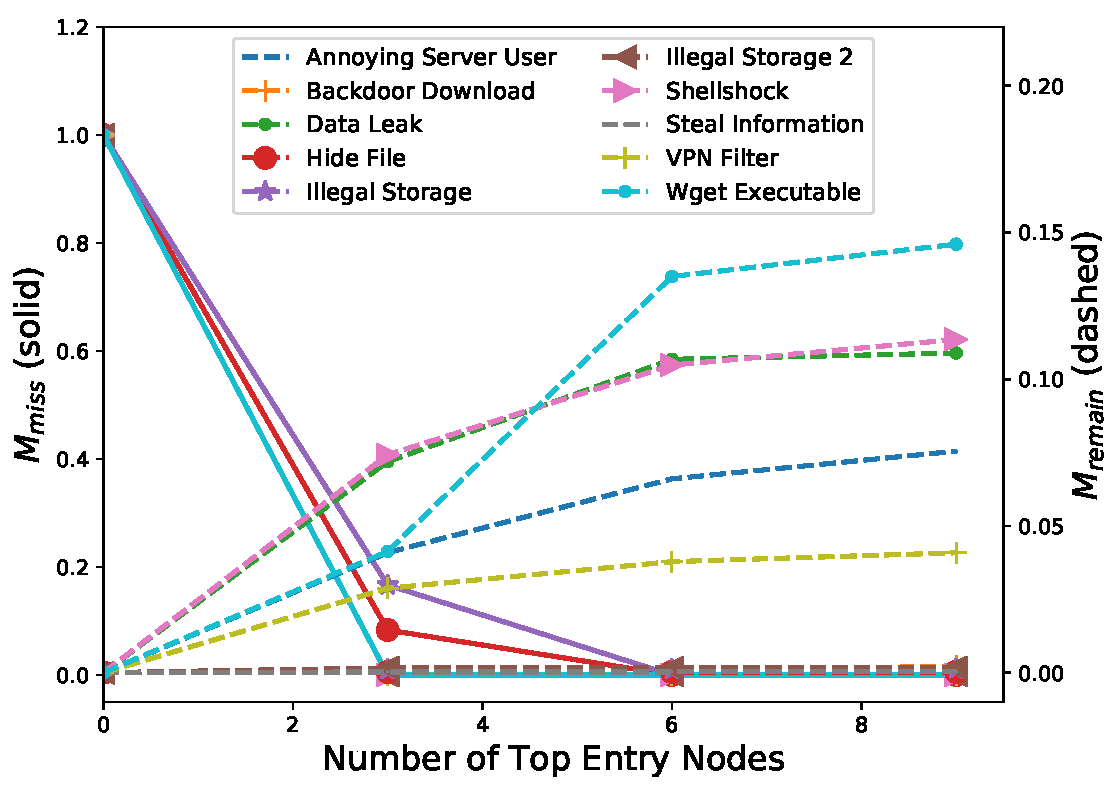
\includegraphics[width=0.47\textwidth]{figs/s&p/rq2-crop.pdf}
    \caption{$M_{miss}$ and $M_{remain}$ using top-ranked entry nodes by considering 3 types of system entities (3, 6, 9 nodes)}
    \label{fig:rq2batch}
\end{figure}
\begin{figure}[t]
    \centering
    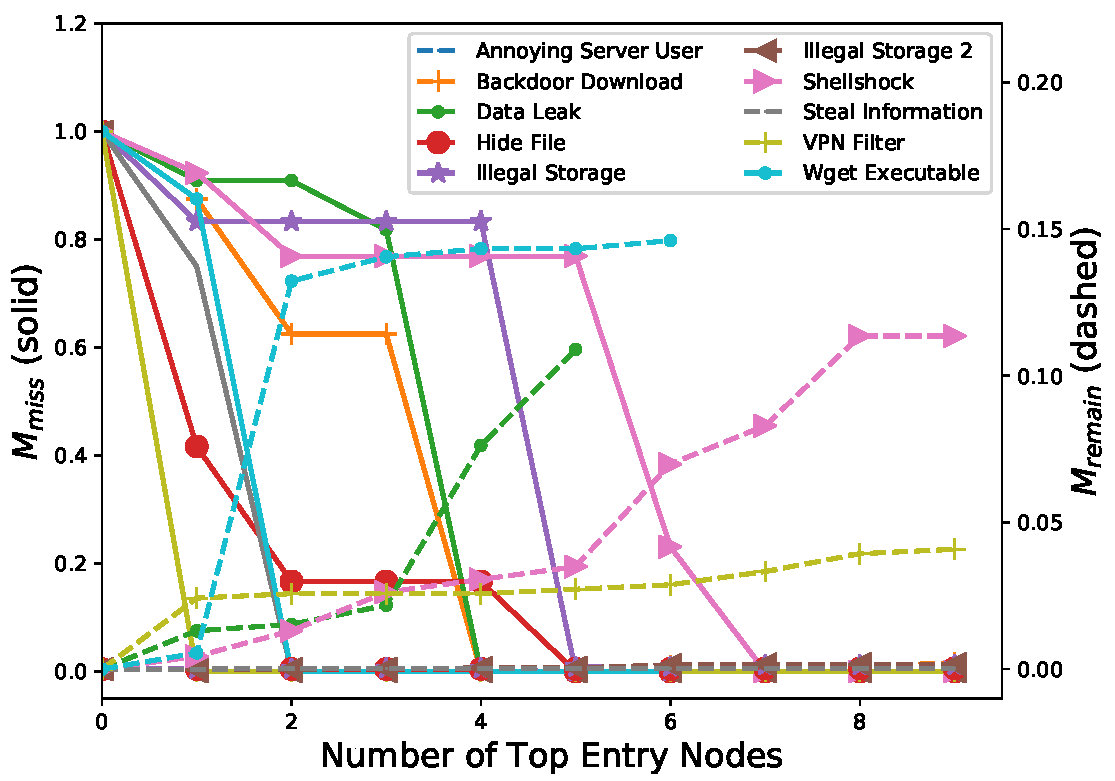
\includegraphics[width=0.47\textwidth]{figs/s&p/rq2m-crop.pdf}
    \caption{$M_{miss}$ and $M_{remain}$ using top-ranked entry nodes without considering the types of system entities (1-9 nodes)}
    \label{fig:rq2single}
\end{figure}

\subsection{RQ2: Impacts of Top-Ranked Entry Nodes}
\label{subsec:rq2}
% Given a dependency graph from a POI event, \tool chooses a number of top-ranked nodes to perform forward causality analysis, and remove the edges that cannot be found via the forward causality analysis.
Intuitively, the more entry nodes \tool uses to perform forward causality analysis, the less likely \tool will incorrectly filter out critical edges.
However, more entry nodes will also cause more non-critical edges to be preserved in the final output graph.
%(\ie overlap of the forward dependency graph and the original backward dependency graph). 
To demonstrate the effectiveness of selecting the top-ranked entry nodes in revealing attack sequences, we show how the increase of the selected top-ranked entry nodes impact the effectiveness of \tool in preserving critical edges and filtering out non-critical edges.
As attack entries may be from different types of system entities, we also compare the effectiveness of two mechanisms in selecting top-ranked entry nodes: one considers the types of system entities and the other does not.

% we first compare \tool with a random approach that randomly selects entry nodes to perform forward causality analysis for filtering. 
% For \tool, we choose top 1, top 2, and top 3 entry nodes from the 3 types of system entities to perform the graph reduction. 
% For the random approach, we choose the 3, 6, and 9 entry nodes for fair comparison.


\myparatight{Evaluation Metrics}
To measure the missing of critical edges, we compute the \emph{missing rate} $M_{miss} = N_{miss} / N_{critical}$, where $N_{miss}$ represents the number of missing critical edges and $N_{critical}$ represents the total number of critical edges (Column ``Critical Edge'' in \cref{tab:stasticalSummary}).
%
To measure the effectiveness of graph reduction, we compute the \emph{remaining rate} $M_{remain} = N_{remain} / N_{total}$, where $N_{remain}$ represents the number of edges in the output graph 
%generated by \tool 
and $N_{total}$ represents the number of edges in the dependency graph after the edge merge (Column ``Edge Mer. \# E'' in \cref{tab:stasticalSummary}).


\eat{
\myparatight{Comparison to Random Approach}
\cref{tab:toolReductionAndMissing} and \cref{tab:rq2random} show the comparison results.
Columns ``1-$M_{miss}$'', ``1-$M_{remain}$'', and ``1-$\# Edge$'' show the average value of $M_{miss}$, the average value of $M_{remain}$, and the average number of edges in the final graph for \tool and the random approach by using the top 1 entry nodes of the 3 types of system entities.
Columns ``2-$M_{miss}$'', ``2-$M_{remain}$'', ``2-$\# Edge$'', ``3-$M_{miss}$'', ``3-$M_{remain}$'', and ``3-$\# Edge$'' show the same metrics for the top 2 and the top 3 entry nodes, respectively. 

As we can see, when the number of entry nodes increases, $M_{miss}$ decreases from $0.02$ to $0.00$ for \tool, but $M_{miss}$ fluctuates for the random approach. 
Another important fact is that when using more entry nodes, the average number of edges remained in the final graph increases from $244.00$ to $268.10$ for \tool, 
while the average number of edges increases from $31,092.21$ to $654,683.47$ for the random approach, which is significantly larger. 
% After the reduction, \tool has about hundreds of edges, but the graph processed by the random approach still has more than 30,000 edges on average. 
Compared with the random approach, \tool can further reduce the edges produced by the random approach by $99.21\%$, $99.96\%$ and $99.95\%$ using the top 1, top 2, and top 3 entry nodes, respectively.
Note that this improvement is not at the cost of losing critical edges for attacks. 
If \tool uses 6 entry nodes (\ie top 2 entry nodes from the 3 system entities), $M_{miss}$ drops to $0.0$.
These results indicates that using irrelevant entry nodes found by the random approach to perform forward causality analysis for filtering is ineffective and may cause the loss of critical edges,
while the top-ranked entry nodes found by \tool contain attack entries so that \tool is effective in revealing attack sequences. 
}

% At the same time, the total number of the edge in the critical component is $268.10$ on average, when \tool uses all the top-three entry nodes. 
% For the random approach, this number is $654,683.47$. 

\myparatight{Impacts on $M_{miss}$ and $M_{remain}$}
As there are 3 types of system entities (\ie processes, files, and network connections), \tool uses the top-ranked entry nodes in different system entity categories
%from all the system entity types 
to perform forward causality analysis (\ie special treatment in \cref{subsubsec:entry-ranking}). 
\cref{fig:rq2batch} shows the values of $M_{miss}$ and $M_{remain}$ with the increases of the used entry nodes.
As expected, when more entry nodes are used, $M_{miss}$ decreases while $M_{remain}$ increases.
This is because performing the forward causality analysis from more entry nodes will make the final graph overlap larger, which is likely to include more critical edges and more non-critical edges. 
We can clearly see that when 6 entry nodes are used (2 nodes from each of the 3 system entity categories), $M_{miss}$ becomes $0.0$.
We further confirm that these 6 entry nodes cover all the attack entries, and more entry nodes merely contribute to the increase of $M_{remain}$.
Another finding is that the dependency impact of the node ranked at the third is about $70\%$ of the top 1 node's dependency impact.
Thus, alternatively, we can use $70\%$ of the top 1 node's dependency impact as the threshold to choose the top-ranked entry nodes for filtering.


\myparatight{Comparison of Two Selection Mechanisms for Top-Ranked Entry Nodes}
We compare \tool's entry node selection mechanism with another mechanism that does not consider system entity categories (\ie selecting top-ranked entry nodes based on their dependency impacts directly).
\cref{fig:rq2single} shows the values of $M_{miss}$ and $M_{remain}$ for this mechanism.
As we can see, for some attacks (\eg the ``VPNFilter'' and ``Wget Executable'' attacks), $M_{miss}$ becomes $0.0$ when the top 1 and the top 2 entry nodes are used,
but some attacks (\eg the ``Shellshock'' attack) requires 7 entry nodes for $M_{miss}$ to become $0.0$.
On the contrary, for all the attacks, the selection mechanism that considers system types can ensure zero-loss of critical edges when 6 entry nodes are used.

\myparatight{Summary}
These results indicate that (1) the top-ranked nodes provided by \tool are effective in preserving critical edges and reducing non-critical edges when the top 2 entry nodes from the 3 types of system entities are used;
(2) the mechanism that considers the types of system entities when choosing the top nodes achieves more stable results for different type of attacks than the one without considering the types of system entities.







\eat{
Considering the complexity of the potential cyberattack, if users want to include more entry points for forward reduction, the change rate of relevance score can be a useful
threshold that may help users select entry node candidates. 
According to our current results, the suggested threshold value for relevance score change is $28\%$. 
That means users can select entry nodes, whose relevance score is bigger than $72\%$ of the highest relevance score in the corresponding category, to do the forward analysis.
}



\eat{

These results demonstrate the superiority of \tool over the random approach,
which is mainly due to the better selection of the entry nodes.
For \tool, the selection of entry nodes is based on the relevance score ranking. 
For the random approach, this selection is a random decision. 
Based on this finding, we can conclude the effectiveness of the graph reduction highly depends on the selection of entry nodes. 


$M_{size}$ is used to measure the graph reduction rate, which is defined as:
\begin{equation}
    M_{size} = \frac{N_{critical}}{N_{merge}}
\end{equation}
$N_{critical}$ is the number of edges in the critical component generated by \tool. $N_{merge}$ is the number of edges after the edge merges. 
A good reduction method should have a small $M_{size}$. If we don't do any graph reduction, $M_{size}$ will be $1.0$.

$M_{miss}$ is used to measure the information loss during the graph reduction. 
Because the corresponding information is represented as edges in dependency graph, we use the critical-edge missing rate to measure the attack information loss. 
$M_{miss}$ is defined as:
\begin{equation}
    M_{miss} = \frac{N_{missing}}{N_{total}}
\end{equation}
$N_{missing}$ is the number of missing critical edges in the critical component generated by \tool. Since we have control over the test environment of these attack cases, we are able to figure out the ground truth of the attack sequences. 
We have the total number of critical edges that should be contained by the critical component, which is represented by $N_{total}$.
Without any filtering, the dependency graph constructed via performing a backward causality analysis from a POI has the $M_{miss}$ being $0.0$.



\tool chooses the top-ranked entry nodes to perform forward causality analysis, and filter the edges that do not appear in the forward causality analysis. 
For this evaluation, we choose the top 3 entry nodes of each category as candidates, and thus we have 9 nodes as candidates in general. 
Given these candidate nodes, we assume that users may pick any of these 9 nodes to perform forward causality analysis for reduction. 
In this evaluation, we use a straightforward way to add entry nodes for forward reduction. 
We add a batch of entry nodes including all 3 kinds of system entities (\ie file, process and IP), the order is according to the rank of relevance score.
Thus, we compute the $M_{size}$ by allowing users to select all top1, top2, or top3 nodes among these candidates, respectively, and then compute $M_{miss}$.


To demonstrate the effectiveness of \tool's graph reduction, we compare \tool with the random  approach. 
For the random approach, all the entry nodes are candidates and the entry nodes used to do the graph reduction are randomly selected. 
We run the random approach for 20 times and compute the average result for these metrics.
For fairness, we will compare the results of \tool and the random approach with the same number of selected nodes, respectively.
}

% We evaluate the graph reduction and critical-edge missing rate, when the attack investigation uses different number of candidates to do the forward reduction. 
% For the dependency graph reduction, if we just simply remove 99.99\% edges of dependency graph, we may have a small graph can be easily analyzed, but it is very possible that we lose all the information about attack. 
% If we only pursue to keep all the attack information, the safest reduction way is just keep all the edges. 
% However, this graph is still too large to be analyzed. 
% The ideal method is try to keep all the critical edges, at the same time remove as much irrelevant edges to POI event as possible.

\begin{table}[t]
\centering
\caption{Average rank of attack entries}
\label{tab:rq3}
\resizebox{0.5\textwidth}{!}{
\begin{tabular}{crrrrr}
\hline
 
\textbf{Attack}        & \multicolumn{1}{c}{\textbf{\tool-{}-}} & \multicolumn{1}{c}{\textbf{\tool-}} & \multicolumn{1}{c}{\textbf{Avg. Proj.}} & \multicolumn{1}{c}{\textbf{Rand.}} & \multicolumn{1}{c}{\textbf{\tool}} \\ \hline
Wget Executable            & 5.50                                     & 12.25                                          & 20.00                                    & 23.45                                    & 5.50                                 \\
Illegal Storage            & 25.00                                    & 13.00                                          & 18.00                                    & 475.99                                   & 7.00                                 \\
Illegal Storage2           & 1.00                                     & 1.00                                           & 1.00                                     & 1,893.66                                 & 1.00                                 \\
Hide File                  & 22.00                                    & 10.50                                          & 13.50                                    & 17,284.72                                & 1.00                                 \\
Steal Information          & 11.00                                    & 3.50                                           & 7.00                                     & 17,304.32                                & 11.00                                \\
Backdoor Download          & 3.50                                     & 3.50                                           & 7.50                                     & 76.57                                    & 6.50                                 \\
Annoying Server User\_user & 5.00                                     & 5.00                                           & 13.00                                    & 15.82                                    & 4.00                                 \\
Shellshcok                 & 11.00                                    & 19.00                                          & 13.00                                    & 22.63                                    & 11.00                                \\
Dataleak                   & 35.00                                    & 9.00                                           & 9.00                                     & 48.34                                    & 8.00                                 \\
VPN Filter                 & 46.00                                    & 34.00                                          & 8.00                                     & 236.77                                   & 7.00                                 \\
Five Dir. Case1            & 5.00                                     & 5.00                                           & 5.00                                     & 115.50                                   & 5                                    \\
Five Dir. Case3            & 1                                        & 1                                              & 1                                        & 327.10                                   & 2                                    \\
Theia Case1                & 1                                        & 1                                              & 1                                        & 88956.7                                  & 1                                    \\
Theia Case3                & 1                                        & 2                                              & 1                                        & 70610.5                                  & 1                                    \\
Trace Case5                & 2                                        & 2                                              & 2                                        & 10.1                                     & 2                                    \\
AVG                        & 11.67                                    & 8.12                                           & 8.00                                     & 13,160.14                                & 4.87                                 \\ \hline
\end{tabular}
}
\end{table}

%\begin{table}[!t]
\centering
\caption{Performance statistics of \tool}
\label{tab:runtime}
\resizebox{0.48\textwidth}{!}{%
\begin{tabular}{|l|r|r|r|r|r|}
\hline
            \textbf{Case}         & \textbf{Causality} & \textbf{Edge Merge} & \textbf{Node Split} & \textbf{Weight} & \textbf{Rep. Propagation} \\ \hline
penetration-c1       & 0.088                     & 0.001           & 0.002             & 0.013                          & 0.069                              \\ \hline
penetration-c2       & 0.086                     & 0.000           & 0.000             & 0.027                          & 0.001                              \\ \hline
password-crack-c1    & 0.186                     & 0.001           & 0.000             & 0.009                          & 0.000                              \\ \hline
password-crack-c2    & 0.183                     & 0.007           & 0.001             & 0.015                          & 0.001                              \\ \hline
password-crack-c3    & 0.256                     & 0.152           & 0.001             & 0.022                          & 0.000                              \\ \hline
data-leakage         & 0.568                     & 0.450           & 0.019             & 1.697                          & 0.031                              \\ \hline
command-injection-c1 & 0.246                     & 0.001           & 0.001             & 0.020                          & 0.000                              \\ \hline
command-injection-c2 & 0.215                     & 0.025           & 0.006             & 0.668                          & 0.008                              \\ \hline
vpnfilter-c1         & 0.179                     & 0.002           & 0.000             & 0.006                          & 0.000                              \\ \hline
vpnfilter-c2         & 0.162                     & 0.007           & 0.000             & 0.053                          & 0.000                              \\ \hline
\textbf{avg}         & \textbf{0.21}            & \textbf{0.06}  & \textbf{0.003}   & \textbf{0.25}                 & \textbf{0.01}                     \\ \hline
\end{tabular}
}
\end{table}


\eat{
\begin{figure}[t]
    \centering
    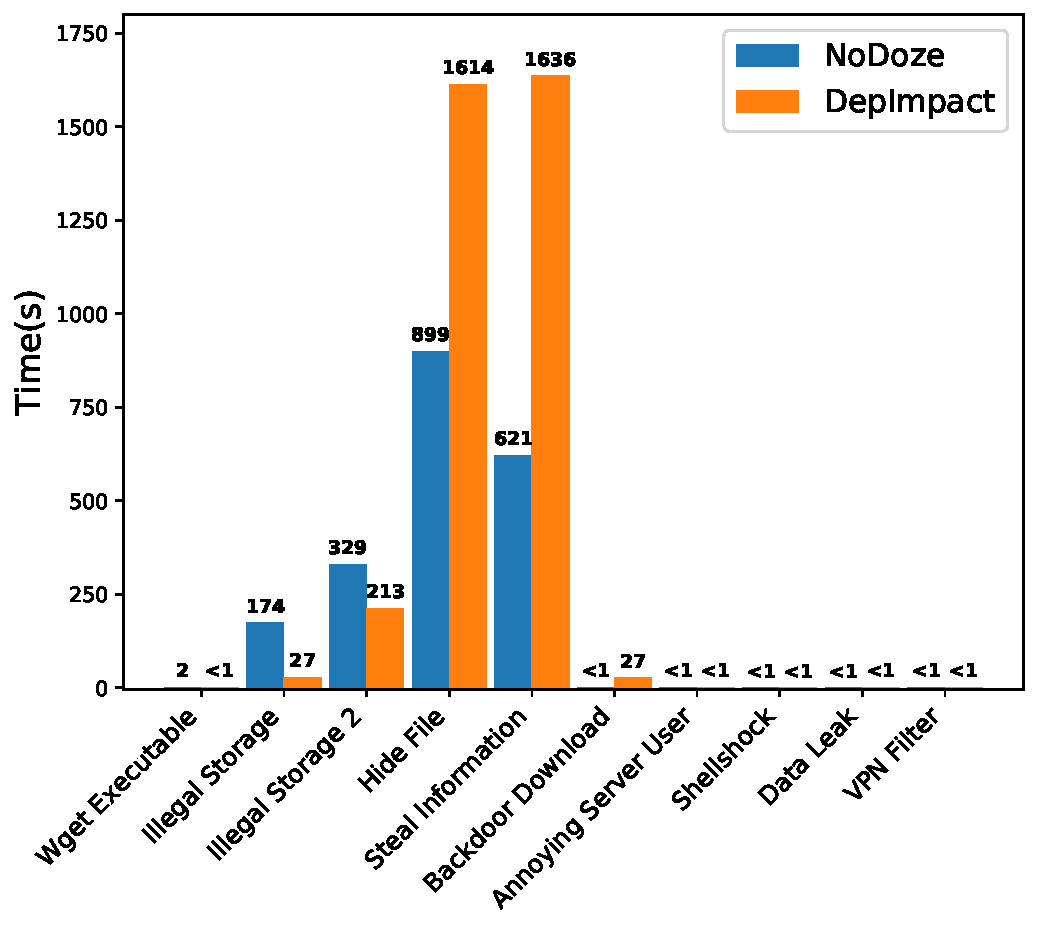
\includegraphics[width=0.48\textwidth]{figs/s&p/rq4.pdf}
    \caption{Runtime performance of \tool and NoDoze}
    \label{fig:rq4compare}
\end{figure}
}

\subsection{RQ4: System Performance}

To understand the performance of \tool, we measure the execution time of each step in \tool, as shown in \cref{tab:rq4performance}.
On average, \tool takes $343.84s$ to finish
%the processing and computation for one 
analyzing an attack (\ie weight computation and impact propagation) and dependency graph construction requires $65.83s$ (\ie causality analysis and edge merge).
We next compare \tool with the average-projection approach and NoDoze.
We exclude the comparison of the execution times for the common steps (causality analysis and edge merge).


% We compare \tool with the average-projection approach for dependency weight computation and dependency impact propagation, since they share the same steps for causality analysis and edge merge. 
From the comparison results of \tool and the average-projection approach in \cref{tab:rq4performance}, we observe that 
(1) \tool takes more time for dependency weight computation ($\sim120s$) because \tool uses the Multi-KMeans++ clustering and LDA to find the optimal projection vector;
(2) \tool takes less time for dependency impact propagation. The reason is because the dependency weights computed by \tool are much more discriminative, and hence the score propagation can converge faster.
%but the shorter time for the average-projection approach in dependency weight computation is offsetted by the time needed for score propagation. 
As a result, \tool reduces the execution time by $71.94\%$ when compared with the average-projection approach. 

% We also compare the execution time of \tool (dependency weight computation plus dependency impact propagation) with the execution time of NoDoze (anomaly score computation), since they share the same causality analysis and edge merge steps. We only compare the different parts: weight computation and impact propagation.
From the comparison results of \tool and Nodoze in \cref{tab:rq4performance}, we can see \tool need $343.84s$ to finish the weight computation and impact propagation, NoDoze need $144.15s$ to finish the s anomaly score computation.
%
In particular, while \tool requires more time for processing the 2 attacks whose dependency graphs have more than 3 million edges (\ie the ``Hide File'' attack and the ``Steal information'' attack), \tool produces much smaller graphs ($\sim800$ edges) than NoDoze ($>20,000$ edges).
On average, \tool needs $343.84$s to finish the dependency weight computation and the dependency impact propagation, and NoDoze needs $144.15$s to finish the anomaly score computation ($409.67s$ v.s. $209.98s$ for the whole analysis).
%
Thus, \tool and NoDoze have similar runtime performance for most of the attacks, and NoDoze is more efficient for certain attacks but achieves much lower graph reduction. 



\eat{
Also, the results in \cref{subsec:rq3} show that \tool achieves better ranking for the attack entries than the average-projection approach, and we want to know whether it is at the cost of more computation efforts.
The results are shown in \cref{tab:rq4performance}.



To understand the performance of \tool in investigating real attacks, we measure the execution time of \tool on the attack cases.
\tool starts the computation by parsing a log ($92.252s$ averagely) and building a global graph representation ($3.277s$ averagely).
\cref{tab:runtime} shows the execution time for the remaining components of \tool. 
Besides the steps shown in the preprocessing step, \emph{Causality Analysis}, \emph{Edge Merge}, and \emph{Node split} require $0.21s$, $0.06s$, and $0.003$ on average. 
Note that \emph{Weight Computation} and \emph{Reputation Propagation} only requires $0.25s$ and $0.01s$ on average.
In summary, the total time for running an analysis is about $2$ minutes, but the major cost (\ie log parsing) can be improved by adopting caching or database indexing~\cite{gao2018aiql}.
}


\eat{
\subsection{Evaluation Summary}
The evaluation results show that \tool is effective in preserving all the critical edges and filtering non-critical edges by choosing the top 2 top-ranked entry nodes to do the forward causality analysis for reduction. 
On average, the size of the graph produced by \tool is only $4.9\%$ of the dependency graph generated by directly applying causality analysis from the POI event. 
Such a great reduction result relies on the proper selection of the top-ranked entry nodes for the forward causality analysis. 
The comparison to 4 other state-of-the-art causality analysis techniques show that \tool is at least 33 times more effective in dependency graph reduction, and does not share the same limitations as these techniques (\eg training on an execution profile and reputation assignment).
Our results also show that \tool consistently ranks the ground-truth sources at the top ($3.13$ on average). 
Finally, \tool finishes analyzing an attack within $8$ minutes, which is slightly slower than the state-of-the-art technique NoDoze ($\sim5$ minutes).
Considering the dependency graph has about $130,000$ edges on average, \tool is highly effective and efficient to reveal the critical edges compared with the manual inspection, which will take much more than $8$ minutes.
}





\section{Discussion}
\label{sec:discussion}

\eat{
\subsection{General Framework for Revealing More Attacks}
\tool provides a general framework to assign weights to dependency edges based on a set of features, 
and computes relevance scores based on edge weights.
Our evaluations have shown the effectiveness of \tool using the features (\cref{subsubsec:feature-extraction}) for the commonly used exploits and real attacks.
To reveal the types of attacks that present different properties, a different set of features that describe these properties can be provided to \tool,
and the discriminative feature projection will be able to automatically compute new weights for revealing the attacks. 
}

\subsection{Adversarial Settings}
As briefly discussed in \cref{subsubsec:feature-extraction}, in practice, the attacker, with some knowledge about the proposed system, may optimize its attack strategy to manipulate the proposed features of certain edges. 
For example, (1) to have a lower temporal relevance feature, the attacker may extend its malicious activities during weeks/months to remain stealth, or (2) to have a lower data size relevance feature, the attacker may perform the exfiltration using multiple processes and each process is only associated with small data size. 
%
However, note that the goal of this work is not to design highly robust features to accurately detect malicious activities, which is an orthogonal research question and is very challenging.
Instead, this work targets the design of an effective approach that identifies parts of dependencies that are actually related to a given POI, which is challenging due to the large imbalance between critical edges and non-critical edges.
%
As shown in \cref{subsubsec:rq1}, directly using the features to identify critical edges can lead to many false positives, which in turn demonstrates that it is fairly challenging to design highly effective features.
In contrast, \tool employs novel methods to take advantage of the noisy features (\ie edge weight computation, relevance score propagation, entry node ranking, forward causality analysis) and achieves a much higher graph reduction rate.
%


%\pgao{First, a given POI might correspond to an event that has no data amount attribute; like a rename system call or an unlink system call for deleting a critical file. }


%\pgao{fanout feature; priotracker => does not prune, but prioritize}



\subsection{Design Alternatives}
For feature extraction, besides the features proposed, the design of \tool supports easy incorporation of other features according to specific forensic investigation needs.
%
For edge weight computation, one alternative is to train a binary classifier using the features and output a probability score as the edge weight.
However, such supervised learning-based approach faces significant limitations in our problem context:
(1) as some of our features are computed with respect to the specific POI, the classification model learned for one type of attack can hardly generalize to other types of attacks with different POIs;
(2) such approach typically requires large amount of training data, while our problem context is highly imbalanced in which critical edges are limited. 
%
Among unsupervised learning-based approaches, approaches based on anomaly detection~\cite{anomalysurvey} could be a substitution for KMeans clustering, and there could be alternatives for LDA to achieve discriminative dimensionality reduction~\cite{Mika99fisherdiscriminant,sugiyama2006local}.
We plan to explore these options in future work.

%\pgao{maybe talk about local clustering approach}


\subsection{Parallel Execution}
Many parts of \tool can be potentially parallelized with distributed computing.
Backward and forward causality analyses can be parallelized by searching the dependency separately. 
Feature extraction for different edges is independent and can be easily parallelized.
%In the scenarios where multiple hosts are involved, dependencies on each host can be precomputed in parallel and thus cross-host causality analysis becomes the concatenation of multiple generated dependency graphs. 
Relevance score propagation (\cref{eq:reputation}) can be converted into a matrix-vector product form to save CPU cycles.
Further parallelization is possible by leveraging ideas similar to parallelizing PageRank~\cite{gleich2004fast,kohlschutter2006efficient}. 
We plan to explore these ideas in future work.



%Weighted causality analysis with parallelization is an interesting research direction that requires non-trivial efforts




\eat{
The construction of
causality graphs can be potentially parallelized with distributed
computing. Any individual branch to be explored can be
processed separately; branches may bear different priorities
and therefore are assigned with corresponding computing
resources; dependencies on each host can also be pre-computed
in parallel and cross-host tracking thus becomes the concatenation of multiple generated graphs. Nonetheless, the massive
and pervasive dependencies among system events bring significant challenges to parallel processing, and therefore distributed
causality tracking by itself is an interesting research direction
that requires non-trivial efforts.
}



\eat{
\subsection{Industrial View}
Because APT attacks consist of many small steps over a long period of time, even though security experts can obtain the system-wide log, it is time-consuming to manually inspect the daunting number of edges in the system dependency graph, and thus it is hard to discover the complete attack steps and reconstruct the attack sequence.
Moreover, depending on the individual's capability, the quality of the analysis may vary a lot. 
By enabling automatic investigation, \tool not only reduces the time consumption of the analysis but also mitigates the dependency on the capability of the security analysts.
This makes \tool highly applicable to small-scale businesses that are not affordable to hire a large team of security analysts to conduct labor-intensive investigation. 
%The automated process is vital to keep the security level as high as possible. 
% In places where there are multiple servers, such as a large-scale business, this work can guarantee a level of security through automation and help security experts to respond promptly. The prompt response will help to reduce the financial damage when a security incident happens.
}


\section{Related Work}
\label{sec:literature}

In this section, we survey three categories of related work.


\myparatight{Forensic Analysis via System Audit Logs}
Significant progress has been made to leverage system-level audit logging for forensic analysis.
%
Causality analysis based on system auditing data plays a critical role.
King et al.~\cite{backtracking,backtracking2} proposed a backward causality analysis technique to perform intrusion analysis by automatically reconstructing a series of events that are dependent on a user-specified POI event.
Goel et al.~\cite{taser} proposed a technique that recovers from an intrusion based on forensic analysis.
%Further
Recent efforts have been made to mitigate the dependency explosion problem by performing fine-grained causality analysis~\cite{beep,ma2016protracer,mcitracking,ji2017rain,ji2018enabling}, prioritizing dependencies~\cite{liu2018priotracker,hassan2019nodoze}, customized kernel~\cite{trustkernel}, and optimizing storage~\cite{loggc,reduction,reduction2,reduction3}. 
However, these techniques suffer from adoption limitations as they mainly rely on heuristic rules that cause loss of information~\cite{backtracking}, intrusive system changes such as binary instrumentation~\cite{ma2016protracer,mcitracking} and kernel customization~\cite{trustkernel}, or execution profiles that have limited generalizations~\cite{hassan2019nodoze}.
\tool proposes to compute discriminative dependency weights based on multiple features and perform back-propagation from the POI event to compute dependency impacts for identifying attack entries, which do not share the same adoption limitations with the existing techniques. 
Our evaluation results further demonstrate the effectiveness of \tool over the existing techniques.
%capture more types of attacks.


Behavior querying leverages domain-specific languages (DSLs) to search for patterns of system call events.
Gao et al.~\cite{gao2018aiql,gao2018saql} proposed a domain-specific languages that enables efficient attack investigation by querying the historical and real-time stream of system call events.
A major limitation of these DSLs is that they require manual efforts to construct the queries, which is labor-intensive and error-prone.
Milajerdi et al.~\cite{HOLMES} propose to rely on the correlation of suspicious information flows to detect ongoing attack campaigns.
They further propose to leverage the knowledge from cyber threat intelligence (CTI) reports to align attack behaviors recored in system auditing data~\cite{poirot}. 
Pasquier et al.~\cite{pasquier2018runtime} propose a runtime analysis of provenance by combining runtime kernel-layer reference monitor with a query module. 
Hossain et al.~\cite{sleuth} propose a tag-based technique to perform real-time attack detection and reconstruction fro system auditing data. 
While the focuses are different, \tool can be interoperated with these techniques to achieve a better defense.

% To reduce the false threat alarms, Hassan et al.~\cite{hassan2019nodoze} proposed to rely on the contextual and historical information of generated threat alert to combat threat alert fatigue.
% automate provenance analysis, reducing large number of false alarms keeping the true attack scenarios. Based on their ranked threats, \tool can further complement their work in revealing attack sequence for the threats. 



% \pgao{Need to add recent publications, sp19, usniex 19, ccs19, sp20}




\eat{
To mitigate the burden of storing large amount of system monitoring data, 
Lee et al.~\cite{loggc} proposed to leverage garbage collection to remove temporary files,
Xu et al.~\cite{reduction} proposed to merge dependencies while still preserving high-fidelity causal dependencies,
and Tang et al.~\cite{reduction2} used templates to summarize the set of system libraries loaded at the process initiation period.
\tool can be 
integrated with these works to achieve better scalability for handling cases that span a long period of time (\eg months).}



\myparatight{Score Propagation}
Our relevance score propagation scheme was inspired by the TrustRank algorithm~\cite{Gyongyi:2004:vldb}, which was originally designed to separate spam and reputable web pages: it first selects a small set of reputable seed pages, then propagates the trust scores following the link structures using the PageRank algorithm~\cite{Page:techreport:1998}, and identifies spam pages as those with low scores. Similar ideas have been applied in security and privacy application scenarios
including Sybil detection~\cite{cao2012sybilrank,Gong:2014:tifs,gao2018sybilfuse}, fake review detection~\cite{Rayana:2015:COS:2783258.2783370}, and attribute inference attacks~\cite{jia2017attriinfer}.
%
\tool is the first work that applies the score propagation idea in system audit logging domain that propagates dependency impacts to identify attack entries for filtering irrelevant dependencies.

% with the focus on reducing the size of dependency graph and identifying relevant dependencies to facilitate forensic investigation.

%the reputation score in an inheritance fashion rather than a distribution fashion, which avoids the serious degradation of reputation scores after propagating on long dependency paths.

%Wang et al.~\cite{wang2018graph} arguments the graph-based security analysis with weighted edges to counter cases with large number of heterogeneous edges. 
%Their approach requires the labels of the nodes to train a model, which is difficult to obtain for the diversified set of the attacks.





\myparatight{Edge Weight Computation}
Several components of \tool are built up on a set of existing techniques. Our edge clustering step is based on Multi-KMeans++~\cite{Arthur:2007:KAC:1283383.1283494}, which optimizes the seed initialization for better clustering quality, compared with the standard KMeans. 
Our discriminative feature projection step is based on Linear Discriminant Analysis (LDA)~\cite{Mika99fisherdiscriminant}, which finds a linear combination of features that characterizes or separates multiple classes of objects. 

%Yet, to apply it in our setting, we extend the standard LDA to handle the challenges including lack of a prior class information, matrix singularity, and limited number of labeled instances. 
\section{Conclusion}
We have presented a novel causality analysis approach, \tool, which builds a weighted dependency graph from system auditing events that record the information of system calls.
\tool is designed to address the two major problems faced by the causality analysis: dependency explosion and non-trivial efforts in graph inspection.
\tool generates three novel types of discriminative features (\ie relative time difference, relative data amount differences, and concentration degree) for the dependencies among system auditing events, and leverage these features to compute weights for each dependency. 
Based on these weights, \tool can surface attack provenance by hiding low weighted edges.
\tool further propagates reputation from the seed nodes in the weighted dependency graph to automatically determine whether the reputation of a target file is similar to untrusted sources, saving the efforts in graph inspection.
The evaluations on representative cases for key system interfaces and steps in real attacks demonstrate the effectiveness of \tool in addressing dependency explosion and graph inspection.

\bibliographystyle{IEEEtranS}
\bibliography{refs}

\end{document}
